\documentclass[a4paper, twocolumn]{article}
\usepackage{packages}
\usepackage{graphicx, float}
\usepackage{multicol}


\newcommand{\ve}[1]{\mathbf{#1}}
%\newcommand{\bra}[1]{\left\langle #1 \right|}
%\newcommand{\ket}[1]{\left| #1 \right\rangle}
\newcommand{\bracket}[2]{\left\langle #1 \middle| #2 \right\rangle}
\newcommand{\bracketOP}[3]{\left\langle #1 \middle| #3 \middle| #2 \right\rangle}

\title{\LARGE HARTREE-FOCK ALGORITHM APPLIED TO A SYSTEM OF TWO TRAPPED ELECTRONS ILLUMINATED THROUGH A LASER SOURCE \\ \vspace{4mm}  \large UNIVERSITY OF OSLO - FYS4411 COURSE \\ \large COMPUTATIONAL PHYSICS II: QUANTUM MECHANICAL SYSTEMS - PROJECT 2 }
\author{\textsc{Emiliano Staffoli, Matteo Zortea, Alexander Ferraro} }
\date{\today}

\begin{document}

\pagenumbering{arabic}
\setcounter{page}{1}

\twocolumn[{
\maketitle
\begin{abstract}
    The main aim of this project was to reproduce the results obtained by Zanghellini et al. in \cite{Zanghellini_2004}: here they exploited the Hartree-Fock equations for the analysis of a system of two interacting electrons trapped in a harmonic oscillator potential and illuminated by a laser source. We accessed the ground state properties by mean of a time-independent solver, implemented using both the generalized and restricted spin representation for the single-particle wavefunctions. Their radial part was expanded using the eigenstates of an harmonic hamiltonian. The convergence features associated to the two representations were also analyzed, highlighting the possibility for the general system to explore lower energy regions. A time-dependent solver was also implemented, but limited to the general representation. All the results in terms of ground state energy, one-body density and overlap integral $\bracket{\Psi(t)}{\Psi(0)}$ (being $\Psi$ the Slater determinant for the system) were consistent with the corresponding estimates contained in the mentioned article. The time dependent dipole operator $\bracketOP{\Psi(t)}{\Psi(t)}{\hat{x}}$ was also analyzed for multiple values of the laser frequency $\omega$.
    
    We proceeded further by evolving the system illuminated by a laser for a limited time $T$, then switching the source off. A Fourier analysis was performed on both the signals $\bracketOP{\Psi(t)}{\Psi(t)}{\hat{x}}$ and $\vert \bracket{\Psi(t)}{\Psi(T)} \vert^2$ considered for $t>T$, revealing the relations between the main peaks in the so-obtained spectra and both the frequency of the harmonic trap $\Omega$ and of the laser $\omega$.
\end{abstract}
\vspace{12mm}
}]


\section{INTRODUCTION}
\label{sec:introduction}
   Quantum many-body physics is a very challenging research field that investigates systems populated by multiple particles interacting between each other. Among its numerous application fields we can find quantum chemistry, condensed matter physics and materials science, which brought to an increasing interest towards this subject in the scientific community. A further push in this direction was provided by the improvement in the computational performance of modern machines achieved in the last decades: this contribution revealed to be fundamental, since the complexity of the treated systems requires computational approaches. 

A quantum many-body problem can be faced with different methods, the choice of which depends on the features of the system in exam. One of the most famous approaches is constituted by the Hartree-Fock method, which was introduced for the first time by Hartree in 1928 \cite{hartree_1928}. Two years later the procedure was generalized independently by Slater \cite{slater} and Fock \cite{fock}, who included in the mathematical treatment the anti-symmetry of the wavefunction required by the Pauli exclusion principle for a system of fermions. The approach essentially allows to find an approximated solution to the Schr\"odinger equation, providing thus with an estimate for both the wavefunction and consequently the energy of the considered system. This is achieved by mean of the minimization of the energy functional with respect to the single-particle wavefunctions: this produces a system of equations in which each particle is under the action of the mean-field potential generated by the others. A self-consistency requirement is then imposed, leading thus to an iterative procedure that returns the single-particle wavefunctions entering in the construction of the Slater determinant for the system.

However, the simple Hartree-Fock method fails when it aims to describe more complex systems, involving for example the dynamics of a group of electrons illuminated by an intense laser source. An attempt to face this lack of accuracy was faced by Zanghellini et al. in \cite{Zanghellini_2003} with the introduction of the so-called multi-configuration time-dependent Hartree-Fock (MCTDHF) method. As suggested by the name, this new approach is based on the adoption of multiple Slater determinants (or configurations) for the description of the system. The accuracy achievable with the introduction of this hypothesis was tested again by Zanghellini et al. in \cite{Zanghellini_2004}: here the MCTDHF was adopted to access the properties of two systems, respectively constituted by a couple of electrons in a harmonic oscillator potential and a Helium atom. In both the cases a time-dependent potential representing an external laser source was also added. \\

In the context of this project, we adopted the standard time-dependent Hartree-Fock method to reproduce the results obtained by Zanghellini et al. for $\eta=1$, namely when just one Slater determinant is employed for the description of the system. Limiting our analysis to the 2-electron case, we first accessed the main features of the apparatus in its ground-state at $t=0$. The so-obtained results served as seed at a later stage, when the time-dependence represented by the laser field in the Hamiltonian was included. Further analysis not directly related to the content of the paper were also conducted: a more detailed description will be provided in the next section. The results were achieved on our side through the implementation of a Python code relying on the modules provided in \cite{gitOyvind}: this library allows us to face the problem by expanding the unknown single-particle wavefunctions in series of eigenstates of the harmonic oscillator (HO) hamiltonian. The task was then reduced to the determination and manipulation of the coefficients entering in this expansion.

\subsection{OVERVIEW OF THE WORKFLOW}
After this brief general introduction, we will proceed in the next section with the description of the main features of our system, together with the theory elements exploited in the context of this project. In particular, we will focus on the derivation of the time-independent and time-dependent Hartree-Fock equations, together with the main aspects behind the Fourier analysis of the time-dependent dipole moment and overlap. Later, Section \ref{sec:methods} introduces the expansion of the single particle states on a properly chosen basis, arriving then to the Ruthaan-Hall equations and their time-dependent generalization. The structure of the code and the main features of the \texttt{quantum-system} library appear in Section \ref{sec:code}, followed then by the description of the results and related discussions respectively in Section \ref{sec:results} and Section \ref{sec:discussion}. Finally, some possible further developments of this project are described in Section \ref{sec:improvements}, concluding then with the main learning points in Section \ref{sec:conclusions}.



\section{THEORY AND MATHEMATICAL INSTRUMENTS}
\label{sec:theory}
    
The treatment of complex many-body systems such as molecules or clusters represents a very demanding task. The introduction of some properly chosen approximations usually leads to a solution for the considered problem, the price to pay being a possible lack of accuracy in the obtained results. Extended systems illuminated by strong laser sources constitute a clear example: they are very complex to treat both computationally and theoretically and even the adoption of the so-called single active electron approximation is of any help in this context \cite{Zanghellini_2004}. Moreover, well known and established methods as the time-dependent Hartree-Fock or the time-dependent density functional theory suffer of a lack of accuracy when applied to the description of electron dynamics in such complex systems \cite{Zanghellini_2004}. Zanghellini et al. tried to provide for a new approach \cite{Zanghellini_2003} to this kind of problems, formulating the so-called Multi-configuration time-dependent Hartree-Fock method for strong laser field problems. As the name suggests, this strategy still relies on the standard Hartree-Fock theory, but now the total wavefunction describing a system of fermions is expanded in a series of Slater determinants. Higher levels of accuracy can be reached as the number of terms $\eta$ in the expansion increases, finally reaching the exact solution for $\eta \rightarrow \infty$. 

At a later stage the validity of the approach was tested by applying it for the description of two systems, the first constituted by two electrons trapped in a harmonic oscillator potential, the second being represented by a He atom. Both the configurations were subject to a strong laser field. Procedures and results are reported in \cite{Zanghellini_2004}: here the attention is mainly focused on determining the number of Slater determinants that allows to reach a convergence with the numerically exact solution to the considered problems. On the contrary, we will limit our discussion to the case $\eta=1$, trying to reproduce the results for the 2-electrons systems only.

\subsection{PRELIMINARY TIME-INDEPENDENT TREATMENT}

\subsubsection{TIME INDEPENDENT HAMILTONIAN}
The first part of the project was devoted to access the main properties of the system in its ground state. According to the content of the article, the following 1-D Hamiltonian was adopted
\begin{align}
\begin{split}
    \mathcal{H}(x,y) =& -\frac{1}{2} \left( \frac{\partial^2}{\partial x^2} + \frac{\partial^2}{\partial y^2} \right) + \frac{1}{2} \Omega^2 (x^2 + y^2) + \\
    & + \frac{1}{\sqrt{(x-y)^2 + a^2}} \\
    =& \sum_{i=1}^2 h_{i}^{ho} + v(x,y)
\end{split}
\label{eq:hamiltonian_t_indep}
\end{align}
where $x$ and $y$ are the coordinates for the two electrons. The single-particle Hamiltonians $h_i^{ho}$ are limited to a kinetic energy term and a harmonic oscillator potential with frequency $\Omega=0.25$, since at this stage the time dependence is still not included. The interaction between the electrons is represented by a smoothed Coulomb potential, where the shielding parameter $a=0.25$ has been inserted to avoid divergences. Notice that the natural units convention has been adopted, namely $\hbar=4\pi\varepsilon_0=m_e=e=1$, thus all the results reported in the project are consequently represented, even if not explicitly specified. \\

\subsubsection{TIME-INDEPENDENT HARTREE-FOCK METHOD}
A good approximation for the wavefunction that minimizes the energy of the system can be accessed by means of the time-independent Hartree-Fock method. The derivation provided in this section mainly refers to \cite{bransden}, in the special case of the ground state of a system populated by $N$ electrons. \\

In a quite general case, the hamiltonian that describes such a system is assumed to be 
\begin{equation*}
    \mathcal{H} = \mathcal{H}_1 + \mathcal{H}_2
\end{equation*}
where $\mathcal{H}_1$ is the single particle hamiltonian (or one body hamiltonian)
\begin{equation*}
    \mathcal{H}_1 = \sum_{i=1}^N h_i = \sum_{i=1}^N -\frac{1}{2}\nabla_{\ve{r}_i}^2 + V(r_i)
\end{equation*}
and $\mathcal{H}_2$ is the interaction term
\begin{equation*}
    \mathcal{H}_2 = \sum_{i<j,j=1}^N v(\vert r_i-r_j \vert)
\end{equation*}
Since we are dealing with a system of fermions, the wavefunction describing the ground state of the system $\Psi(q_1, \dots, q_N)$ must be antisymmetric under the action of the permutation operator $P$ so that
\begin{gather*}
    P_{ij} \Psi(q_1, \dots,q_i, \dots, q_j, \dots, q_N) = \\
    = \Psi(q_1, \dots, q_j, \dots, q_i, \dots, q_N) = \\ 
    = - \Psi(q_1, \dots, q_i, \dots, q_j, \dots, q_N) 
\end{gather*}
The central idea of the method consists in assuming that the ground state wavefunction $\Psi(q) \equiv \Psi(q_1, \dots, q_N)$ can be approximated by a Slater determinant of single particle wavefunctions
\begin{equation*}
    \Psi(q) \approx \Phi(q) \equiv \frac{1}{\sqrt{N!}} \ \begin{vmatrix} \phi_{1}(q_1) \ \phi_{2}(q_1) \ \dots \ \phi_{N}(q_1) \\ 
    \phi_{1}(q_2) \ \phi_{2}(q_2) \ \dots \ \phi_{N}(q_2) \\
    \dots \\
    \dots \\
    \dots \\
    \phi_{1}(q_N) \ \phi_{2}(q_N) \ \dots \ \phi_{N}(q_N)
    \end{vmatrix}
\end{equation*}
and then make use of the variational principle
\begin{equation}
    \bracketOP{\Psi}{\Psi}{\mathcal{H}} = \mathbb{E}[\Psi] \leq \mathbb{E}[\Phi] = \bracketOP{\Phi}{\Phi}{\mathcal{H}}
    \label{eq:en_ground_slater_1}
\end{equation}
to find the single particle functions $\phi_{1}, \dots \phi_{N}$ that minimize the expectation value of the energy $\mathbb{E}[\Phi]$. \\ Each of the numerical subscripts used in the definition of $\Phi$ refers to a particular set of quantum numbers $(n_1, n_2, n_3, ...)$ so that the notation $\phi_{i}(q_k)$ stands for the single electron orbital identified by the set of quantum numbers $i = (n_1^i, n_2^i, n_3^i, ...)$ evaluated in the position of the particle $k$. Notice that index $i$ runs over the single-particle states, while $k$ runs over the particles, both ranging from 1 to N. We also require that ${\phi_{i}(q_k)}$ is an orthonormal basis set, so that $\langle \phi_{i}|\phi_{j}\rangle =\delta_{i, j} $ .

The approximated wavefunction can be rewritten by making use of the antisymmetrizer operator $\mathcal{A}$, whose properties are described in \cite{bransden}:

\begin{equation}
\begin{aligned}
    \Phi(q) &= \frac{1}{\sqrt{N!}}\bigg(\sum_P (-1)^P \hat{P} \bigg) \Phi_H(q) \\
     &= \sqrt{N!} \, \mathcal{A} \, \Phi_H(q)
\end{aligned}
\label{eq:slater_determinant}
\end{equation}
where $\hat{P}$ indicates the permutation operator and $\Phi_H(q)$ is:
\begin{equation*}
    \Phi_H(q) = \phi_1(q_1) \, \phi_2(q_2) \, \dots \, \phi_N(q_N)  
\end{equation*}
Using the variational principle one can estimate the energy of the ground state with the initial guess on $\Phi$. Starting from Eq.\,\ref{eq:en_ground_slater_1}, it follows that
\begin{align*}
    \mathbb{E}[\Phi] &= \bracketOP{\Phi}{\Phi}{\mathcal{H}} \\
    &= \bracketOP{\Phi}{\Phi}{\mathcal{H}_1} + \bracketOP{\Phi}{\Phi}{\mathcal{H}_2}
\end{align*}
Let us study the $\mathcal{H}_1$ term. Exploiting the fact that $[\mathcal{A}, H_1]=0$, $\mathcal{A}^2 = \mathcal{A}$ and the hermiticity of the operator, one gets 
\begin{align*}
    \bracketOP{\Phi}{\Phi}{\mathcal{H}_1} &= N! \bracketOP{\Phi_H}{\Phi_H}{\mathcal{A}\mathcal{H}_1 \mathcal{A}} \\
    &= N! \bracketOP{\Phi_H}{\Phi_H}{\mathcal{H}_1\mathcal{A}^2} \\
    &= N! \bracketOP{\Phi_H}{\Phi_H}{\mathcal{H}_1\mathcal{A}} \\
    &= \sum_{i=1}^N \sum_P (-1)^P \bracketOP{\Phi_H}{\Phi_H}{h_i\hat{P}} 
\end{align*}
In the last sum over the possible permutations, the only term that survives is obtained when the permutation operator coincides with the identity operator (see Appendix A). This happens because we choose an orthonormal basis set for $\phi_i(q)$, yielding to: 
\begin{align}
    \bracketOP{\Phi}{\Phi}{\mathcal{H}_1} &= \sum_{i=1}^N  \bracketOP{\Phi_H}{\Phi_H}{h_i}
    \label{eq:permutation_to_identity}
\end{align}
which in turn becomes a sum over the $N$ individual quantum states
\begin{align*}
    &= \sum_{i} \bracketOP{\phi_i}{\phi_i}{h} = \sum_{i} I_i
\end{align*}
We indicated with $I_i$ the average value of the individual hamiltonian $h$ evaluated on the the spin orbital $\phi_i$.

Now we focus on the $\mathcal{H}_2$ interaction term: exploiting the fact that $[\mathcal{A}, \mathcal{H}_2]=0$, $\mathcal{A}^2 = \mathcal{A}$ and the hermiticity of the operator one gets
\begin{align*}
    \bracketOP{\Phi}{\Phi}{\mathcal{H}_2} &= N! \bracketOP{\Phi_H}{\Phi_H}{\mathcal{A} \mathcal{H}_2 \mathcal{A}} \\
    &= N! \bracketOP{\Phi_H}{\Phi_H}{\mathcal{H}_2 \mathcal{A}} \\
    &= \sum_P (-1)^P  \bracketOP{\Phi_H}{\Phi_H}{\mathcal{H}_2 P} \\
    &= \sum_{i<j} \sum_P (-1)^P  \bracketOP{\Phi_H}{\Phi_H}{v(r_{ij}) P}
\end{align*}
where $r_{ij}=|r_i -r_j|$. The orthonormality of the single-particle wavefunctions leads us to say that the only non-zero terms are those obtained when the operator $P$ coincides with the identity or when $P$ exchanges the indexes $i \leftrightarrow j$ (this follows from an analogous reasoning to that reported in Appendix A):   
\begin{align*}
    &= \sum_{i<j} \bracketOP{\Phi_H}{\Phi_H}{v(r_{ij})(1-P_{ij})}
\end{align*}
Again, the sum over $i<j$ can be rewritten as a sum over the individual quantum states, obtaining at the end
\begin{align*}
    &= \frac{1}{2} \sum_{i,j} \bigg\{ \bracketOP{\phi_i (q_1) \phi_j(q_2)}{\phi_i (q_1) \phi_j (q_2)}{v(r_{12})} - \\
    & - \bracketOP{\phi_i (q_1) \phi_j(q_2)}{\phi_j (q_1) \phi_i (q_2)}{v(r_{12})} \bigg\} \\
    &= \frac{1}{2} \sum_{i,j} \bigg\{ \bracketOP{\phi_i \phi_j}{\phi_i \phi_j }{v(r_{12})} - \bracketOP{\phi_i \phi_j}{\phi_j \phi_i }{v(r_{12})} \bigg\} \\
    &= \frac{1}{2} \sum_{i,j} \bigg\{ \mathcal{F}_{ij} - \mathcal{K}_{ij} \bigg\}
\end{align*}
where $\mathcal{F}_{ij}$ and $\mathcal{K}_{ij}$ are defined respectively as the direct and exchange term. Joining the results obtained up to now, one gets that
\begin{align}
    \mathbb{E}[\Psi] = \sum_i I_i + \frac{1}{2} \sum_{i,j} \mathcal{F}_{ij} - \mathcal{K}_{ij}
    \label{eq:expected_val_energy}
\end{align}
At this point one can proceed with the minimization of the energy functional with respect to the single-particle states. The orthonormality condition for these functions is taken into account by introducing $N^2$ Lagrange multipliers, obtaining then
\begin{align}
    \delta E - \sum_{ij} \varepsilon_{ij} \delta \langle \phi_i \vert \phi_j \rangle = 0
    \label{eq:lag_mult_interm_step}
\end{align}
We notice that the number of independent element inside the matrix of the Lagrange multipliers is actually reduced to $N(N-1)/2$, this due to the redundancy in the imposition of the same condition on $\langle \phi_i \vert \phi_j \rangle$ and $\langle \phi_j \vert \phi_i \rangle$. In particular, this leads to the hermiticity of the matrix, since $\varepsilon_{ij}^* = \varepsilon_{ji}$. It is known that a hermitian matrix can always be diagonalized through a proper basis change operated by a unitary matrix $U$, thus we shall assume that $\{\phi_i\}_{i=1}^N$ actually corresponds to the so-obtained basis. We notice that this basis change does not influence the procedures described up to now, since the full wavefunction gains at most a phase factor. Eq.\,\ref{eq:lag_mult_interm_step} then reduces to
\begin{align*}
    \delta E - \sum_{ij} \varepsilon_{i} \delta_{ij} \delta \langle \phi_i \vert \phi_j \rangle = 0
\end{align*}
the result of which becomes a system of single particle equations, namely
\begin{align}
\begin{split}
     &h_i \phi_i(q_1) + \bigg[ \sum_j \int dq_2 \phi_j^*(q_2) v(r_{12}) \phi_j(q_2) \bigg] \phi_i (q_1) - \\
    & - \sum_j \int dq_2 \phi_j^*(q_2) v(r_{12}) \phi_i(q_2) \bigg] \phi_j (q_1) = \varepsilon_i \phi_i (q_1)
\end{split}
\label{eq:fock_matrix_t_ind}
\end{align}
where the sums are performed over the occupied molecular orbitals. The direct term appearing in each equation accounts for the fact that each particle is moving in the average potential generated by the presence of the others in the system. In this sense the Hartree-Fock methods is operating in a mean-field approximation. The presence of the exchange term is on the contrary a pure quantum effect, which derives from the assumption made on the total wavefunction $\Psi$ to be written as a Slater determinant. For the sake of completeness, we introduce also the so-called Fock operator, which allows to rewrite the equation above as
\begin{align*}
    \hat{f} \phi_i = \varepsilon_i \phi_i
\end{align*}
From an operative point of view, one starts from an initial guess for each $\phi_i$ and then proceeds by feeding at each step the equations just reported with the single particle wavefunctions obtained at the previous iteration. The procedure continues ideally until the self-consistency requirement has been fulfilled, namely up to the point in which the various $\phi_i$ become the exact eigenstates of Hartree-Fock equations, with $\varepsilon_i$ being the corresponding eigenvalues. 



\subsubsection{EXPECTATION VALUES}
The results in terms of total wavefunction $\Psi$ provided at the end of the iterative process can be used to access some important properties of the system in its ground state. Adapting the results to the actual apparatus, we recall from Eq.\,\ref{eq:expected_val_energy} that the total energy can be achieved as
\begin{align}
\begin{split}
    \mathbb{E}[\mathcal{H}] &= \sum_{i=1}^2 \bracketOP{\phi_i}{\phi_i}{h^{ho}} + \frac{1}{2} \sum_{i,j=1}^2 \bigg\{ \bracketOP{\phi_i \phi_j}{\phi_i \phi_j }{v(x,y)} - \\
    &- \bracketOP{\phi_i \phi_j}{\phi_j \phi_i }{v(x,y)} \bigg\} 
\end{split}
\label{eq:total_energy_no_coeff}
\end{align}
while the ground-state one-body density comes from the following definition 
\begin{align}
\begin{split}
    \rho(x) =& \int [dy] \Psi^*(x,y) \Psi(x,y) \\
    =& \sum_{i=1}^N \sum_{\sigma} \vert \phi_i(x; \sigma) \vert^2
\end{split}
\label{eq:one_body_density_no_coeff}
\end{align}
This last equality can be derived again exploiting the properties of the anti-simmetrization operator entering in the definition of $\Phi$. Notice that with the notation $[dy]$ we are including also the bra-ket between the spin components $\sigma$ contained into each single particle wavefunctions. This operation is represented by the sum over $\sigma$ in the last step.


\subsection{TIME-DEPENDENT TREATMENT}
\subsubsection{TIME-DEPENDENT HAMILTONIAN}
After a first stage described above, the time-dependence in the Hamiltonian can now be included. This is made by introducing the potential term describing the action of the laser field to which the system is subjected, namely
\begin{align}
\begin{split}
    H(x,y; t) =& -\frac{1}{2} \left( \frac{\partial^2}{\partial x^2} + \frac{\partial^2}{\partial y^2} \right) + \frac{1}{2} \Omega^2 (x^2 + y^2) + \\
    &+ \frac{1}{\sqrt{(x-y)^2 + a^2}} + (x+y) \fakeeps_0 \sin (\omega t) \\
    =& \sum_{i=1}^2 h_i' + v(x,y) \\
    =& \sum_{i=1}^2 \left[ h_i^{ho} + h_{i}^{L} \right]+ v(x,y)
\end{split}
\label{eq:hamiltonian_t_dip}
\end{align}
where $x$ and $y$ stand again for the coordinates for the two electrons. Now the single-particle terms have been enriched with the presence of the time-dependent sinusoidal contribution, where $\omega=8 \Omega = 2$ and $\fakeeps_0 = 1$.


\subsubsection{TIME-DEPENDENT HARTREE-FOCK METHOD}
The introduction of a temporal factor in the Hamiltonian requires the adoption of the time-dependent version of the method derived above. In the time dependent case, the approximated ground state wavefunction $\Psi(t, q)$ can be deduced by the principle of minimum action which reads
\begin{equation*}
    \delta \mathcal{S}[\Psi, \Psi^*] = 0
\end{equation*}
for a suitable choice of the action $\mathcal{S}[\Psi, \Psi^*]$. In the following derivation we assume the action to be of the form
\begin{equation*}
    \mathcal{S}[\Psi, \Psi^*, \lambda] = \int_{t_0}^t \mathcal{L}(\Psi, \Psi^*, \lambda) \, dt'
\end{equation*}
with $\mathcal{L}(\Psi, \Psi^*, \lambda)$ Lagrangian function given by
\begin{equation}
\begin{gathered}
    \mathcal{L}[\Psi, \Psi^*, \lambda] = \left\langle\Psi(t)\left|\mathfrak{i \hbar} \partial_{t}-\mathcal{H}(t)\right| \Psi(t)\right\rangle
\end{gathered}
\label{eq:lagrangian_def}
\end{equation}
In light of the definition provided for the action functional, its minimization condition reduces to 
\begin{align}
\begin{split}
    &\delta\mathcal{S}[\Psi, \Psi^*, \lambda] = \int_{t_0}^t \delta \mathcal{L}(\Psi, \Psi^*, \lambda) \, dt' = 0 \qquad \Rightarrow \\
    & \Rightarrow \qquad \mathcal{L}(\Psi, \Tilde{\Psi}^*, \lambda) -  \mathcal{L}(\Psi, \Psi^*, \lambda) = 0
\end{split}
\label{eq:minimiz_action}
\end{align}
where the term $\Tilde{\Psi}$ simply corresponds to a variation on the total wavefunction that will be described in a moment.

As for the time independent case, the true wavefunction $\Psi(t, q)$ is approximated by a function $\Phi(t, q)$ constructed as a Slater determinant as in Eq.\,\ref{eq:slater_determinant}. Thus the terms in the Lagrangian in Eq.\,\ref{eq:lagrangian_def} can be expanded using this assumption. This brings to a new form for the Lagrangian, namely
\begin{equation*}
\begin{gathered}
    \mathcal{L}[\Phi, \Phi^*, \lambda] = \left\langle\Phi(t)\left| i \partial_{t}-\mathcal{H}(t)\right| \Phi(t)\right\rangle + \\ - \sum_{i,j} \lambda_{ji}\left(\left\langle\phi_{i}(i) \mid \phi_{j} (t) \right\rangle-\delta_{ij}\right)
\end{gathered}
\end{equation*}
where we have introduced the Lagrange multipliers $\lambda_{ij}$ to account for the orthogonality of the single particle states. \\
The previously mentioned variation on the total wavefunction can then be performed by introducing a variation on one single particle state per time
\begin{equation*}
    \widetilde \phi_i(t, q_i) = \phi_i(t, q_i) + \delta_{ik} \epsilon \eta(t, q_i) 
\end{equation*}
where $\epsilon$ is regarded as a real parameter and $\eta(t, q_i)$ is a complex valued function. Note that, as before, the variations on $\phi_i$ and $\phi_i^*$ (or, analogously on the ket $\ket{\phi_i}$ and on the bra $\bra{\phi_i}$) can be treated as independent. \\

At this point, we can proceed with the explicit evaluation of the expression for $\mathcal{L}[\Phi, \widetilde\Psi ^*, \lambda]$. Let us proceed by following the scheme proposed for the time-independent case. Notice that now the time-dependences will be omitted for the sake of simplifying the notation.
\begin{align*}
    \bracketOP{\widetilde\Phi}{\Phi}{\mathcal{H}_1} 
    &= \sum_{i=1}^N \sum_P (-1)^P \bracketOP{\widetilde\Phi_H}{\Phi_H}{h_i\hat{P}} \\
    &= \sum_{i=1}^N \bracketOP{\widetilde\phi_i}{\phi_i}{h} \\
    &= \sum_{i=1}^N \bracketOP{\phi_i}{\phi_i}{h} + \epsilon \sum_{i=1}^N \bracketOP{\eta}{\phi_i}{h} \delta_{ik} \\
    &= \sum_{i=1}^N \mathcal{I}_i(t) + \epsilon \bracketOP{\eta}{\phi_k}{h} 
\end{align*}
Notice that the hermiticity of the operator $i\partial_t$ allows to treat it as a single-particle operator. This result will be included later. Similarly, the 2-body term becomes
\begin{align*}
    &\bracketOP{\Phi}{\Phi}{\mathcal{H}_2}
    = \sum_{i<j} \bracketOP{\widetilde\Phi_H}{\Phi_H}{v(r_{ij})(1-P_{ij})} \\
    &= \frac{1}{2} \sum_{i,j} \bigg\{ \mathcal{F}_{ij}(t) - \mathcal{K}_{ij}(t) \bigg\} + \\
    &\quad +\epsilon \frac{1}{2} \sum_{i,j} \bigg\{ \delta_{ik} \bracketOP{\eta \phi_j}{\phi_i \phi_j }{v(r_{12})}_{AS} + \\
    & \quad + \delta_{jk} \bracketOP{\phi_i \eta}{\phi_i \phi_j }{v(r_{12})}_{AS} \bigg\} \\ 
    &= \frac{1}{2} \sum_{i,j} \bigg\{ \mathcal{F}_{ij}(t) - \mathcal{K}_{ij}(t) \bigg\} + \epsilon \sum_{i} \bracketOP{\eta \phi_i}{\phi_k \phi_i }{v(r_{12})}_{AS}
\end{align*}
The evaluation of the expression for $\mathcal{L}[\Phi, \Phi^*, \lambda]$ just adds the time dependence to the expressions obtained in the time-independent case.\\

Joining all the results that we got up to now, we get
\begin{align*}
    &\mathcal{L}(\Psi, \Tilde{\Psi}^*, \lambda) -  \mathcal{L}(\Psi, \Psi^*, \lambda) = \\
    & = i\epsilon \bracketOP{\eta}{\phi_k}{\partial_t} - \epsilon \bracketOP{\eta}{\phi_k}{h} - \epsilon \sum_{i} \bracketOP{\eta \phi_i}{\phi_k \phi_i }{v(r_{12})}_{AS} - \\
    & \quad- \epsilon \sum_j \lambda_{kj} \bracket{\eta}{\phi_j} \\
    &= i\epsilon \bracketOP{\eta}{\phi_k}{\partial_t} - \epsilon \bracketOP{\eta}{\phi_k}{\hat{f}(t)} - \epsilon \sum_j \lambda_{kj} \bracket{\eta}{\phi_j} = 0
\end{align*}
where we have introduced the time-dependent version of the Fock operator. Since the function $\eta$ was arbitrarily chosen, the result of the previous equation must not depend on its form, thus we get
\begin{align*}
    i \partial_t \ket{\phi_k} - \hat{f}(t) \ket{\phi_k} - \sum_j \lambda_{kj} \ket{\phi_j} = 0
\end{align*}
The expression for the generic Lagrange multiplier follows by projecting the result onto $\phi_l$.
\begin{align*}
    \bracketOP{\phi_l}{\phi_k}{i\partial_t} - \bracketOP{\phi_l}{\phi_k}{\hat{f}(t)} = \sum_j \lambda_{kj} \delta_{jl} = \lambda_{kl}
\end{align*}
Substituting the result for $\lambda_{kj}$ into the last equation, we get
\begin{gather*}
    i \partial_t \ket{\phi_k} - \hat{f}(t) \ket{\phi_k} - \sum_j \left[ \bracketOP{\phi_j}{\phi_k}{i\partial_t} - f_{jk} \right] \ket{\phi_j} = 0
\end{gather*}
which after the introduction of the operator $\mathds{P}$ can be rewritten as
\begin{align}
    \underbrace{ \left( \hat{\mathbb{1}} - \sum_j \ket{\phi_j} \bra{\phi_j} \right)}_{\hat{\mathds{P}}}  \left[ i\partial_t \ket{\phi_k} - \hat{f}(t) \ket{\phi_k} \right] = 0
    \label{eq:intermed_step_t_dep_HF}
\end{align}
% Notice that the sum appearing in the definition of the operator $\mathds{P}$ does not lead to a completeness relation, since $\{ \phi_j \}_{j=1}^N$ do not form a complete basis. \\
At this point, we can consider an arbitrary hermitian operator $\hat{Q}(t)$ and apply a unitary transformation to the single-particle states that makes this equation true
\begin{equation*}
    \bracketOP{\phi_p}{\phi_q}{i \partial_t} = \bracketOP{\phi_p}{\phi_q}{\hat{Q}(t)}
\end{equation*}
where $\phi_p$ and $\phi_q$ have to be intended as the transformed single particle states. The unitary transformation does not invalidate all the results applied up to now, since the Slater determinant gains at most a phase factor and the Lagrangian remains unaltered. The operator $\hat{Q}(t)$ was chosen arbitrarily, with the only requirement of being Hermitian, thus it can be set equal to $\hat{f}(t)$. After the single-particle state have undergone the proper unitary transformation, the following equation will then be satisfied
\begin{equation*}
    \bracketOP{\phi_p}{\phi_q}{i \partial_t} = \bracketOP{\phi_p}{\phi_q}{\hat{f}(t)}
\end{equation*}
Returning to Eq.\,\ref{eq:intermed_step_t_dep_HF} and inserting this last result, we finally get the time-dependent version of the Hartree-Fock equations
\begin{align*}
    &i\partial_t \ket{\phi_k} - \hat{f}(t) \ket{\phi_k} - \sum_j \ket{\phi_j} \left[ \bracketOP{\phi_j}{\phi_k}{i\partial_t} - \bracketOP{\phi_j}{\phi_k}{\hat{f}(t)} \right] \\
    &= i\partial_t \ket{\phi_k} - \hat{f}(t) \ket{\phi_k} - \sum_j \ket{\phi_j} \left[ \cancel{f_{jk}(t)} - \cancel{f_{jk}(t)} \right] = 0 \;\; \Rightarrow \\
    &\Rightarrow \qquad i\partial_t \ket{\phi_k} - \hat{f}(t) \ket{\phi_k} = 0
\end{align*}
In coordinate representation, this becomes
\begin{equation}
    i \frac{\partial }{\partial t} \phi_i(x;t) = \hat{f}(t) \phi_i(x;t)
    \label{eq:HF_eq_time_dep}
\end{equation}\\
The new form of the Hartree-Fock equations still works in the context of mean-field approximation, but now the action of the operator $\hat{f}$ provides us with the time derivative of the single-particle wavefunctions, rather than with some kind of eigenvalue. Solving the time-dependent Hartree-Fock equations allows then to access the evolution in time of the single particle states. The initial conditions for the solution of the present system of equations are provided by the the single-particle wavefunctions obtained after the convergence of the Hartree-Fock equations in the time-independent treatment. 

\subsubsection{EXPECTATION VALUES}
A good parameter that provides a feedback on the modifications that the individual particle states encounter during their evolution is constituted by the overlap between the total wavefunction at two different instants. Considering $t=0$ as the reference, the indicator assumes the following value
\begin{align}
    \xi(t) = \langle \Psi(x,y; t) \vert \Psi(x,y; 0) \rangle 
    \label{eq:overlap_no_coeff}
\end{align}
then the smaller the value of $\xi$, the smaller the similarities between the wavefunctions describing the system respectively at $t=0$ and $t>0$. 

The effect brought by the introduction of the time-dependent potential associated to the laser appears also in the average displacement of the particles with respect to the center of the system. The evolution in time of this quantity can be evaluated as
\begin{align}\begin{split}
    \overline{x}(t) &= \bracketOP{\Psi(x,y; t)}{\Psi(x,y; t)}{\hat{x}} \\
    &= \sum_{i=1}^N \bracketOP{\phi_i(x;\sigma)}{\phi_i(x; \sigma)}{\hat{x}}
\end{split}
\label{eq:x_time_dep_no_coeff}
\end{align}
%Ti piace di più così o come era prima?


\subsection{FOURIER ANALYSIS}
\label{sec:intro_fourier}
The time evolution of the position operator $\hat{x}$ just described can be used to estimate the transition energy between the ground state and the excited states of the system under exam. In fact, considering an apparatus in its ground state at time $t=0$ described by an Hamiltonian $H_0$, one can apply a time-dependent perturbation with a finite duration $T$ and then return to the original time-independent description. The total wavefunction at time $T$ can then be written as a linear combination of the eigenstates $\Psi_i$ of $H_0$, namely
\begin{align*}
    \ket{\Psi(t>T)} &= \sum_i c_i(t) \ket{\Psi_i}  \\
    &= \sum_i \e^{-iH_0 (t-T)}  c_i(T) \ket{\Psi_i} \\
    &= \sum_i \e^{-i E_i (t-T)} c_i(T) \ket{\Psi_i}
\end{align*}
Here we used the fact that, since $H_0$ is time-independent, the time-evolution of the various excited states is simply provided by the operator $\exp ( -iH_0t)$. Using this formalism, we can rewrite the time-dependence in $\overline{x}(t)$ defined in Eq.\,\ref{eq:x_time_dep_no_coeff} as
\begin{align}
    \overline{x}(t-T) &= \bracketOP{\Psi(t-T)}{\Psi(t-T)}{\hat{x}} \nonumber \\
    &= \sum_{i,j} c_i^*(t) c_j(t) \bracketOP{\Psi_i}{\Psi_i}{\hat{x}} \nonumber \\
    &= \sum_{i,j} \e^{i [E_i - E_j] (t-T)} c_i^*(T) c_j(T)  \bracketOP{\Psi_i}{\Psi_i}{\hat{x}} \nonumber \\
    &= \sum_{i,j} \e^{i \omega_{ij} (t-T)} c_i^*(T) c_j(T) \bracketOP{\Psi_i}{\Psi_i}{\hat{x}}
    \label{eq:transition_energies}
\end{align}
From this result it is evident that the frequency components entering in $\overline{x}(t)$ stand for the transition energy between the various eigenstates of $H_0$.  \\

Another way to estimate such transition frequencies consists in applying the same procedure to $\vert \braket{\Psi(t)}{\Psi(T)} \vert^2$ for $t>T$. In this case, with the same reasoning described above, one gets
\begin{align*}
    & \xi_T(t)=  \\
    &= \sum_i \vert c_i(T) \vert^4 + \sum_{i\neq j} \vert c_i(T) \vert^2 \vert c_j(T) \vert^2 \cos((E_i - E_j)t)
\end{align*}
Here we exploited some trigonometrical identities (see Appendix B), obtaining that the overlap reduces to a constant term and a sum of sinusoidal functions with frequencies given again by the transition energies between the excited states of the system described by $H_0$. 
   
\section{METHODS}
\label{sec:methods}
    \subsection{HARMONIC OSCILLATOR BASIS AND SPIN}
The problem posed by the Hartree-Fock equations can be faced through the choice of a proper basis to represent the single-particle wavefunctions. For what concerns the radial part of the individual states, the presence of the harmonic oscillator term in the Hamiltonians of Eq.\,\ref{eq:hamiltonian_t_indep} and Eq.\,\ref{eq:hamiltonian_t_dip} suggests the employment of the corresponding harmonic oscillator eigenstates, namely
\begin{align*}
    &\hat{h} \chi_{\Tilde{\mu}} (x) = \left[ -\frac{1}{2} \frac{\partial^2}{\partial x^2} + \frac{1}{2} \Omega^2 x^2 \right] \chi_{\Tilde{\mu}}(x) = \varepsilon_{\Tilde{\mu}}^{ho} \chi_{\Tilde{\mu}}(x) \\
    &\varepsilon_{\Tilde{\mu}} (x) = \left( \frac{\Omega}{\pi} \right)^{1/4} \frac{1}{\sqrt{2^{{\Tilde{\mu}}}  {\Tilde{\mu}}!}} H_\mu(\sqrt{\Omega}x) \\
    &\varepsilon_{\Tilde{\mu}}^{ho} = \Omega \left( {\Tilde{\mu}} + \frac{1}{2} \right)
\end{align*}
where $H_{\Tilde{\mu}}(x)$ are the Hermite polynomials and ${\Tilde{\mu}}=1,\dots,l$, being $l$ the number of basis elements that we choose for the representation. 

Since we are dealing with a system of fermions, the spin plays a fundamental role too and must be included in the treatment. While Zanghellini et al. employed the unrestricted representation, we opted for the general ansatz, namely the single particle wavefunction takes the form of a spinor \cite{state_of_art}. The basis elements then become
\begin{align*}
    \vert \psi_\mu \rangle = \vert \chi_{\mu//2} \rangle \otimes \vert \sigma \rangle
\end{align*}
where $\mu=1,\dots,2l$, since the introduction of spin components obviously doubled the number of basis elements. Calling $\alpha$ and $\beta$ respectively the spin-up and spin-down spinors, we precise that $\sigma=\alpha$ for even $\mu$ values, while $\sigma=\beta$ for odd $\mu$ values.

In light of these facts, a single-particle state can be expanded as
\begin{align*}
    \vert \phi_i \rangle = \sum_{\mu=1}^{2l} C_{\mu,i} \vert \psi_\mu \rangle
\end{align*}
which in its extended form corresponds to 
\begin{align}
\begin{split}
    \phi_i(x,m_s) =& \sum_{\Tilde{\mu}=1}^l C_{2\Tilde{\mu},i} \chi_{\Tilde{\mu}}(x) \alpha(m_s) + \\
    +& \sum_{\Tilde{\mu}=1}^l C_{2\Tilde{\mu}+1,i} \chi_{\Tilde{\mu}}(x) \beta(m_s)
\end{split}
\label{eq:expansion_spf_gen}
\end{align}


\subsubsection{NEW FORM OF MATRIX ELEMENTS}
As a result of the introduction of the new basis, it is convenient to represent on the basis itself the matrix elements appearing in the Hartree-Fock equations. Notice that in the following expressions we will use $\Tilde{\mu} = \mu//2$. We introduce the $h^{ho}$ matrix containing the various brakets enclosing the harmonic oscillator hamiltonian as
\begin{align}
    h_{\mu\nu}^{ho} &= \bracketOP{\psi_\mu}{\psi_\nu}{\hat{h} \otimes \hat{\mathbb{1}}} = \bracketOP{\chi_{\Tilde{\mu}}}{\chi_{\Tilde{\nu}}}{\hat{h}^{ho}} \bracket{\sigma_{\mu}}{\sigma_{\nu}} = \nonumber \\
    &= \int dx \chi_{\Tilde{\mu}}(x) \hat{h}^{ho}(x) \chi_{\Tilde{\nu}}(x) \bracket{\sigma_{\mu}}{\sigma_{\nu}} \nonumber \\
    &= \varepsilon_{\Tilde{\mu}}^{ho} \delta_{\Tilde{\mu} \Tilde{\nu} } \bracket{\sigma_{\mu}}{\sigma_{\nu}}  = \varepsilon_{\Tilde{\mu}}^{ho} \delta_{\mu \nu} 
    \label{eq:h_elements}
\end{align}
where the bracket $\bracket{\sigma_{\mu}}{\sigma_{\nu}}$ stands for the dot product between the spin components associated to $\psi_\mu$ and $\psi_\nu$. Similarly, the expected values for the position operator are enclosed in $d$-matrix as
\begin{align}
    x_{\mu\nu} &= \bracketOP{\psi_\mu}{\psi_\nu}{\hat{x} \otimes \hat{\mathbb{1}}} = 
    \bracketOP{\chi_{\Tilde{\mu}}}{\chi_{\Tilde{\nu}}}{\hat{x}} \braket{\sigma_\mu}{\sigma_\nu} \nonumber \\
    &= \int dx \chi_{\Tilde{\mu}}(x) \hat{x} \chi_{\Tilde{\nu}}(x) \bracket{\sigma_{\mu}}{\sigma_{\nu}} 
    \label{eq:x_elements}
\end{align}
These matrix elements will be useful while solving the time-dependent problem, since the potential introduced by the presence of the laser is strictly related to the dipole matrix. Proceeding, the direct and exchange terms appearing in the Hartee-Fock equations are represented as a 4-dimensional matrix $u$ as
\begin{align}
    u^{\alpha\beta}_{\mu\nu} &= \bracketOP{\psi_{\alpha} \psi_{\beta}}{\psi_{\mu} \psi_{\nu}}{v(x,y)} \nonumber \\
    &= \bracketOP{\chi_{\Tilde{\alpha}} \chi_{\Tilde{\beta}}}{\chi_{\Tilde{\mu}} \chi_{\Tilde{\nu}}}{v(x,y)} \bracket{\sigma_{\alpha}}{\sigma_{\mu}} \bracket{\sigma_{\beta}}{\sigma_{\nu}} \nonumber \\
    &= \bigg\{\int dr_1 dr_2 \chi_{\Tilde{\alpha}}^*(r_1) \chi_{\Tilde{\beta}}^* (r_2) v(r_1,r_2) \chi_{\Tilde{\mu}} (r_1) \chi_{\Tilde{\nu}} (r_2) \bigg\} \times\nonumber  \\
    &\times \bracket{\sigma_{\alpha}}{\sigma_{\mu}} \bracket{\sigma_{\beta}}{\sigma_{\nu}} 
    \label{eq:u_elements}
\end{align}
The matrix elements that actually enters in the Hartree-Fock equations are represented by the anti-symmetrized version of $u$, defined as
\begin{align*}
    u^{\alpha\beta}_{\mu\nu,AS} = u^{\alpha\beta}_{\mu\nu} - u^{\alpha\beta}_{\nu\mu}
\end{align*}
In general, we notice that all the matrices introduced up to now share the fact of having null elements in correspondence of indexes whose sum gives an odd number. This follows as a consequence of the convention previously chosen for the labelling of the basis functions, namely even and odd indices are respectively associated with up and down spin components. 



\subsection{ROOTHAAN-HALL EQUATIONS AND THEIR TIME-DEPENDENT GENERALIZATION}
The introduction of the new basis gives new shape also to the Hartree-Fock equations. Considering first the time-independent approach, we restart by substituting each molecular orbital with the corresponding expansion into Eq.\,\ref{eq:fock_matrix_t_ind}, obtaining
\begin{align*}
    &\hat{h} \sum_{\beta} C_{\beta,i} \ket{\psi_\beta} + \sum_{j}^{occ} \sum_{\beta\gamma\delta} C_{\gamma,j}^* C_{\delta,j} C_{\beta,i} \bracketOP{\psi_\gamma}{\psi_\delta}{v(r_{12})} \ket{\psi_\beta} - \\
    &- \sum_{j}^{occ} \sum_{\beta\gamma\delta} C_{\gamma,j}^* C_{\delta,j} C_{\beta,i} \bracketOP{\psi_\gamma}{\psi_\beta}{v(r_{12})} \ket{\psi_\delta} \\
    &= \varepsilon_{i} \sum_{\beta} C_{\beta,i} \ket{\psi_\beta}
\end{align*}
Projecting everything on $\bra{\psi_\alpha}$, one gets
\begin{align*}
    & \sum_{\beta} h_{\alpha,\beta} C_{\beta,i} + \sum_{j}^{occ} \sum_{\beta\gamma\delta} C_{\gamma,j}^* C_{\delta,j} C_{\beta,i} u^{\alpha\gamma}_{\beta\delta,AS} =  \varepsilon_{i}  C_{\beta,i}
\end{align*}
Recurring then to the rewritten form of the Fock matrix elements in the new basis, namely
\begin{align*}
    f_{\mu\nu} =  h_{\mu\nu}^{ho} + \sum_{j}^{occ} \sum_{\gamma\delta} C_{\gamma,j}^* C_{\delta,j} u^{\mu\gamma}_{\nu\delta,AS}
\end{align*}
one can also rewrite the previous system of equations in terms of a matrix product
\begin{align*}
    C\varepsilon = fC
\end{align*}
known also as Roothan-Hall equations. As previously introduced, these have to be cyclically solved up to the reaching of the self-consistency condition. For a numerical approach, this requirement is translated into the following
\begin{align}
    \Delta = \frac{1}{2l} \sum_{k=1}^{2l} \vert \varepsilon_k^{i+1} - \varepsilon_k^i \vert  < \delta
    \label{eq:stop_condition}
\end{align}
where $\varepsilon^{i+1}$ and $\varepsilon^{i}$ are the vectors of eigenvalues provided by the diagonalization of the Fock matrix at two consecutive iterations, while $\delta$ is a parameter chosen by the user. When the condition is satisfied, the algorithm stops.

A similar procedure to obtain the Fock matrix elements can be applied also to the time-dependent Hartree-Fock problem. Considering the result of Eq.\,\ref{eq:HF_eq_time_dep}, one can perform once more the expansion of each molecular orbital and project the so-obtained result onto $\bra{\psi_\alpha}$, getting then
\begin{align*}
    \dot{C}(t) = -i f(t)C(t) 
\end{align*}
where the time-dependent Fock matrix elements are
\begin{align*}
    f_{\mu\nu}(t) =  h_{\mu\nu}^{ho} + x_{\mu\nu} \fakeeps_0 \sin(\omega t) + \sum_{j}^{occ} \sum_{\gamma\delta} C_{\gamma,j}^* C_{\delta,j} u^{\mu\gamma}_{\nu\delta,AS}
\end{align*}




\subsection{INTEGRATOR FOR TIME EVOLUTION}
\label{sec:integrator}
The result of the last equation provides us with the receipe for the time evolution of the system. At every time step the product between the Fock matrix evaluated at time $t$ and the corresponding coefficient matrix gives us the time derivative for each coefficient. The configuration at the following step can the be derived by mean of a properly chosen integrator. For the considered problem we opted for \texttt{zvode} method included in the \texttt{scipy.integrate.ode} \cite{scipy.int} module provided by Python. This choice was driven by the fact that the selected integrator is actually symplectic: this property in our context can be translated in better energy conservation features provided by the integrator itself, and thus an improved physical accuracy in the obtained results. 



\subsection{NEW FORM FOR EXPECTATION VALUES}
The expectation values that we aim to evaluate in this project can also be rewritten in a more convenient form after having performed the basis change. The total energy of the system from Eq.\,\ref{eq:total_energy_no_coeff} becomes
\begin{align}
\begin{split}
    \mathbb{E}[\mathcal{H}] &= \sum_{i=1}^2 \sum_{\alpha,\beta} C_{\alpha,i}^* C_{\beta,i} h_{\alpha\beta}^{ho} + \\
    & + \frac{1}{2} \sum_{i,j=1}^2 \sum_{\alpha\beta\gamma\delta} C_{\alpha,i}^* C_{\gamma,j}^* C_{\beta,i} C_{\delta,j}  u^{\alpha\gamma}_{\beta\delta,AS}
\end{split}
\label{eq:total_energy_coeff}
\end{align}
while the one body density in Eq.\,\ref{eq:one_body_density_no_coeff} is rewritable as
\begin{align}
\begin{split}
    \rho(x) = \sum_i^{occ} \sum_{\alpha\beta} C_{\alpha,i}^* C_{\beta,i} \chi_{\Tilde{\alpha}}^*(x) \chi_{\Tilde{\beta}}(x)
\end{split}
\label{eq:one_body_density_coeff}
\end{align}
The time-dependent overlap appearing in Eq.\,\ref{eq:overlap_no_coeff} then becomes
\begin{align}
    \xi(t) = \big\vert \det \left( C_o^{\dag}(t) C_o(0) \right) \big\vert^2 
    \label{eq:overlap_coeff}
\end{align}
and the corresponding version translated in time is then
\begin{equation}
    \xi_T(t) = \big\vert \det \left( C_o^{\dag}(t) C_o(T) \right) \big\vert^2
    \label{eq:overlap_T_coeff}
\end{equation}
This will be used during the Fourier analysis of the overlap curve. Here we defined $C_o(t)$ as a $2l\times2$ matrix corresponding to the first two columns of the coefficient matrix at time $t$. The number of columns that one has to consider corresponds to the number of particles populating the system. Finally the time-dependent average displacement of Eq.\,\ref{eq:x_time_dep_no_coeff} becomes
\begin{align}
    \overline{x}(t) = \sum_i^{occ} \sum_{\alpha\beta} C_{\alpha,i}^*(t) C_{\beta,i} (t) \bracketOP{\chi_{\Tilde{\alpha}}(x)}{\chi_{\Tilde{\beta}}(x)}{\hat{x}} 
    \label{eq:x_time_dependent_coeff}
\end{align}



\subsection{RESTRICTED HARTREE-FOCK IMPLEMENTATION}
\label{sec:restricted_HF}
At a later stage of the project, we included in our code also the restricted representation of the spin part of the single particle wavefunctions, which then appeared to be written as
\begin{align}
    \phi_i(x,m_s) = \sum_{\mu=1}^{l} C_{\mu,i} \chi_\mu(x) \sigma_{i}(m_s)
    \label{eq:expansion_spf_res}
\end{align}
Here $\sigma$ accounts for the spin component, being $\sigma_i=\alpha$ for $i$ even. The restricted implementation was tested only to find the solution of the ground-state problem in terms of energy and one-body density, excluding then the analysis in the time domain. This allowed us for a comparison with the corresponding results obtained with the general representation described above, especially for what concerns the convergence properties in the time-independent treatment. Here we will limit to briefly describe the modifications brought by the restricted representation in the equations derived above. A full derivation can however be found in \cite{modern_qc}. 

In this context it is no more necessary to employ a basis constituted by $2l$ states, since the spin component is pre-assigned to every single particle wavefunction. Our task is then reduced to identify the $l$ coefficients which enter in the expansion of the radial part of each wavefunction, keeping in mind that each radial part is then associated to two different single particle states with opposite spins. Each sum performed over $\psi_i$ appearing in the previous derivation of the Hartree-Fock equations is then splitted into two restricted sums on the spin-up and spin-down single particle states, namely
\begin{align*}
    \sum_i^N \qquad \rightarrow \qquad \sum_{i,\ket{\uparrow}}^{N/2} + \sum_{i,\ket{\downarrow}}^{N/2}
\end{align*}
Applying all these conditions to the Hartree-Fock equations previously derived, one gets the Fock matrices rewritten in the formalism of the restricted spin representation
\begin{align*}
    f_{\mu\nu} =  h_{\mu\nu}^{ho} + 2\sum_{j}^{n/2} \sum_{\gamma\delta} C_{\gamma,j}^* C_{\delta,j} u^{\mu\gamma}_{\nu\delta} - \sum_{j}^{n/2} \sum_{\gamma\delta} C_{\gamma,j}^* C_{\delta,j} u^{\mu\gamma}_{\delta\nu}
\end{align*}
where $n$ is the number of particles. Notice that the indexes of all the matrices appearing in the equation run from $1$ to $l$, contrarily to what happened in the generalized representation where they could span from $1$ to $2l$. 

The form of the total energy of the system becomes
\begin{align*}
    \mathbb{E}[\mathcal{H}] =& 2\sum_{i=1}^{n/2} \sum_{\alpha,\beta} C_{\alpha,i}^* C_{\beta,i} h_{\alpha\beta}^{ho} + \\
    & + 2 \sum_{i,j=1}^{n/2} \sum_{\alpha\beta\gamma\delta} C_{\alpha,i}^* C_{\gamma,j}^* C_{\beta,i} C_{\delta,j}  u^{\alpha\gamma}_{\beta\delta} - \\
    & - \sum_{i,j=1}^{n/2} \sum_{\alpha\beta\gamma\delta} C_{\alpha,i}^* C_{\gamma,j}^* C_{\beta,i} C_{\delta,j}  u^{\alpha\gamma}_{\delta\beta}
\end{align*}
while the one-body density appears as
\begin{align*}
    \rho(x) = 2 \sum_i^{n/2} \sum_{\alpha\beta} C_{\alpha,i}^* C_{\beta,i} \chi_{\alpha}^*(x) \chi_{\beta}(x)
\end{align*}



\subsubsection{FOURIER ANALYSIS}
\label{sec:fourier_analysis}
For the purpose of estimating the transition energy values as described in Section \ref{sec:intro_fourier}, the time-dependence was introduced in the system by mean of the mentioned laser potential, acting on the apparatus initially in its ground state. The source was left active for a time $T$, then switched off, still proceeding with the time evolution of the system (now in a superposition of eigenstates of the original Hamiltonian). Finally, a Fast Fourier Transform was performed on the so-obtained $\overline{x}(t)$ and $\xi_T(t)$ for $t>T$, extrapolating the frequencies corresponding to the transition energies.




    
\section{CODE STRUCTURE}
\label{sec:code}
\afterpage{
\begin{figure}[H]
\centering
    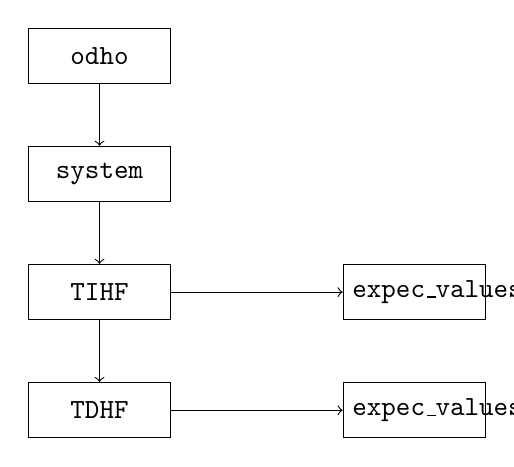
\begin{tikzpicture}
        %[draw, line width=0.3mm, text width=0.13\textwidth, minimum height=30pt, text centered]
        
        \node (odho) [draw, text width=0.13\textwidth, minimum height=20pt, text centered] at (4,0) {\bfseries \texttt{odho}};
        \node (system) [draw, text width=0.13\textwidth, minimum height=20pt, text centered] at (4, -1.5) {\texttt{system}};
        \node (TIHF) [draw, text width=0.13\textwidth, minimum height=20pt, text centered] at (4, -3) { \texttt{TIHF}};
        \node (TDHF) [draw, text width=0.13\textwidth, minimum height=20pt, text centered] at (4, -4.5) { \texttt{TDHF}};
        
        \node (expvalueTIHF) [draw, text width=0.13\textwidth, minimum height=20pt, text centered] at (8, -3) {\texttt{expec\_values}};
        \node (expvalueTDHF) [draw, text width=0.13\textwidth, minimum height=20pt, text centered] at (8, -4.5) { \texttt{expec\_values}};
        
        \draw [->, to path={-| (\tikztotarget)}] (odho.south) -- (system.north);
        \draw [->, to path={-| (\tikztotarget)}] (system.south) -- (TIHF.north);
        \draw [->, to path={-| (\tikztotarget)}] (TIHF.south) -- (TDHF.north);
        \draw [->, to path={-| (\tikztotarget)}] (TIHF.east) -- (expvalueTIHF.west);
        \draw [->, to path={-| (\tikztotarget)}] (TDHF.east) -- (expvalueTDHF.west);
        
    \end{tikzpicture}
    \caption{Diagram describing the workflow behind the implemented code. The \texttt{odho} object is employed for the costruction of the \texttt{system}, which then provides the instruments for the time-dependent and time-independent solvers.}
    \label{diag:code_structure}
\end{figure}
}
We chose Python as a programming language for this project. 
Our program is developed as a Jupyter Notebook, while all the functions and the information on the considered systems are enclosed in a class defined on a separated Python file.
Employing a class for the considered problem allows us to escape from the need of passing many parameters to the implemented functions, using instead the attributes of the class as global variables.

The creator implemented inside the class builds the system, which then can be manipulated and time-evolved by mean of functions defined in the same framework.
The entire program is based on the functions provided in the \texttt{quantum-system} library \cite{gitOyvind}.
This uses finite-difference methods to solve a one-body Hamiltonian $h$ for an arbitrary potential of the form $V(r_i)$, which for our case was chosen to be the harmonic one with frequency $\Omega$. Considering the general representation of the spin, when the creator is called an \texttt{odho} object is built: it contains the first $l$ eigenstates evaluated on a mesh and the corresponding bra-kets appearing in Eq.s \ref{eq:h_elements}, \ref{eq:x_elements} and \ref{eq:u_elements} evaluated between all the possible combinations of the eigenstates. The so-built basis set is then used for the construction of the actual \texttt{system}, namely including the general spin treatment in the problem. The number of basis functions is doubled, with even indexes referring to the spin-up components and odd indexes to the spin-down counterparts. The dimensions of all the matrixes previously mentioned are doubled too. 

After the creation of the system, functions implemented within the class allow to solve the Hartree-Fock equations both with and without the laser source. Other functions take as input the so-obtained coefficients matrix for the ground state to evaluate the expected values presented in the previous sections. Alternatively they can be exploited to proceed with the time evolution of the system and perform the various tasks required for the project. \\

A subclass was implemented for the restricted representation of the spin: here the same reasoning described above applies too, but the attribute \texttt{system} actually coincides with the mentioned \texttt{odho}, since, as seen also in Section \ref{sec:restricted_HF}, the problem can be solved without doubling the number of basis functions to allow for spin mixing.


\begin{minted}[frame=lines, bgcolor=lemonchiffon]{python}
import needed_packages 

class GHF():
    def __init__():
        odho = ODQD([args])
        self.system = 
            GeneralOrbitalSystem([args])
    
    # time-independent HF solver
    def solve_TIHF([args])
    
    # time-dependent HF solver
    def solve_TDHF([args])
    
    # other functions
    def functions()

class RHF(GHF):
    def __init__():
        self.system = ODQD([args])
    
    # adapts some functions from GHF to the
    # RHF case
    def functions_changed()
    
\end{minted}

 



\section{RESULTS}
\label{sec:results}
The main purpose behind this project was to reproduce the results obtained by Zanghellini et al. for a 2-electron interacting system inserted in a harmonic oscillator potential illuminated by a laser source. First we will present the results obtained for the time-independent treatment, switching then to the time-dependent case at a later stage. For the whole development of the code, the radial part of the single particle wavefunctions was written using the first $l=10$ eigenstates $\chi_\mu$ of the harmonic oscillator hamiltonian, entering into Eq.\,\ref{eq:expansion_spf_gen} and Eq.\,\ref{eq:expansion_spf_res}. Each $\chi_\mu$ was evaluated on a mesh of 201 points covering the interval (-10, 10), as specified in the mentioned article. All the results reported below were derived by imposing the initial coefficient matrix equal to an identity matrix with proper dimensionality, namely $2l\times 2l$ and $l\times l$ respectively for the general and restricted solvers. We recall that the natural units convention has been employed, thus all the results reported below are represented in these reduced units.


\subsection{TIME-INDEPENDENT TREATMENT}
As introduced above, the comparison with the results by Zanghellini et al. regarded two main features of the system's ground state, which are the energy and the one-body density. We started by solving the Ruthaan-Hall equations with $\delta=10^{-6}$, adopting both the general and restricted Hartree-Fock solvers. The so-obtained coefficients for the ground state were exploited for the evaluation of the energy and the expected value for the position operator, defined respectively in Eq.\,\ref{eq:total_energy_coeff} and \ref{eq:x_time_dependent_coeff}. The corresponding estimations are reported in Table \ref{tab:E_x_comp_article}. The one-body density was also evaluated and a comparison with the result reported in the article can be found in Figure \ref{fig:one_body_density_comp}. The integral performed over these curves provided us with the values reported again in Table \ref{tab:E_x_comp_article} 

\begin{table}[h!]
    \centering
    \begin{tabular}{cccc}
        \toprule
         & Energy [Hartr.] & Dipole [a.u.] & Integral  \\
        \midrule
        Article & $1.1795$ & - & - \\
        General & $1.17957$ &  $3.539\times10^{-10}$ & $2.000$ \\
        Restric. & $1.17957$ & $1.660\times10^{-10}$ & $2.000$ \\
        \bottomrule
    \end{tabular}
    \caption{Expected values for energy and position operator in the ground state obtained by Zangellini et al. and through our code. Both the general and restricted implementation were exploited, with $\delta=10^{-6}$ and $\Omega=0.25$. }
    \label{tab:E_x_comp_article}
\end{table}



\begin{figure*}[h!]
    \centering
    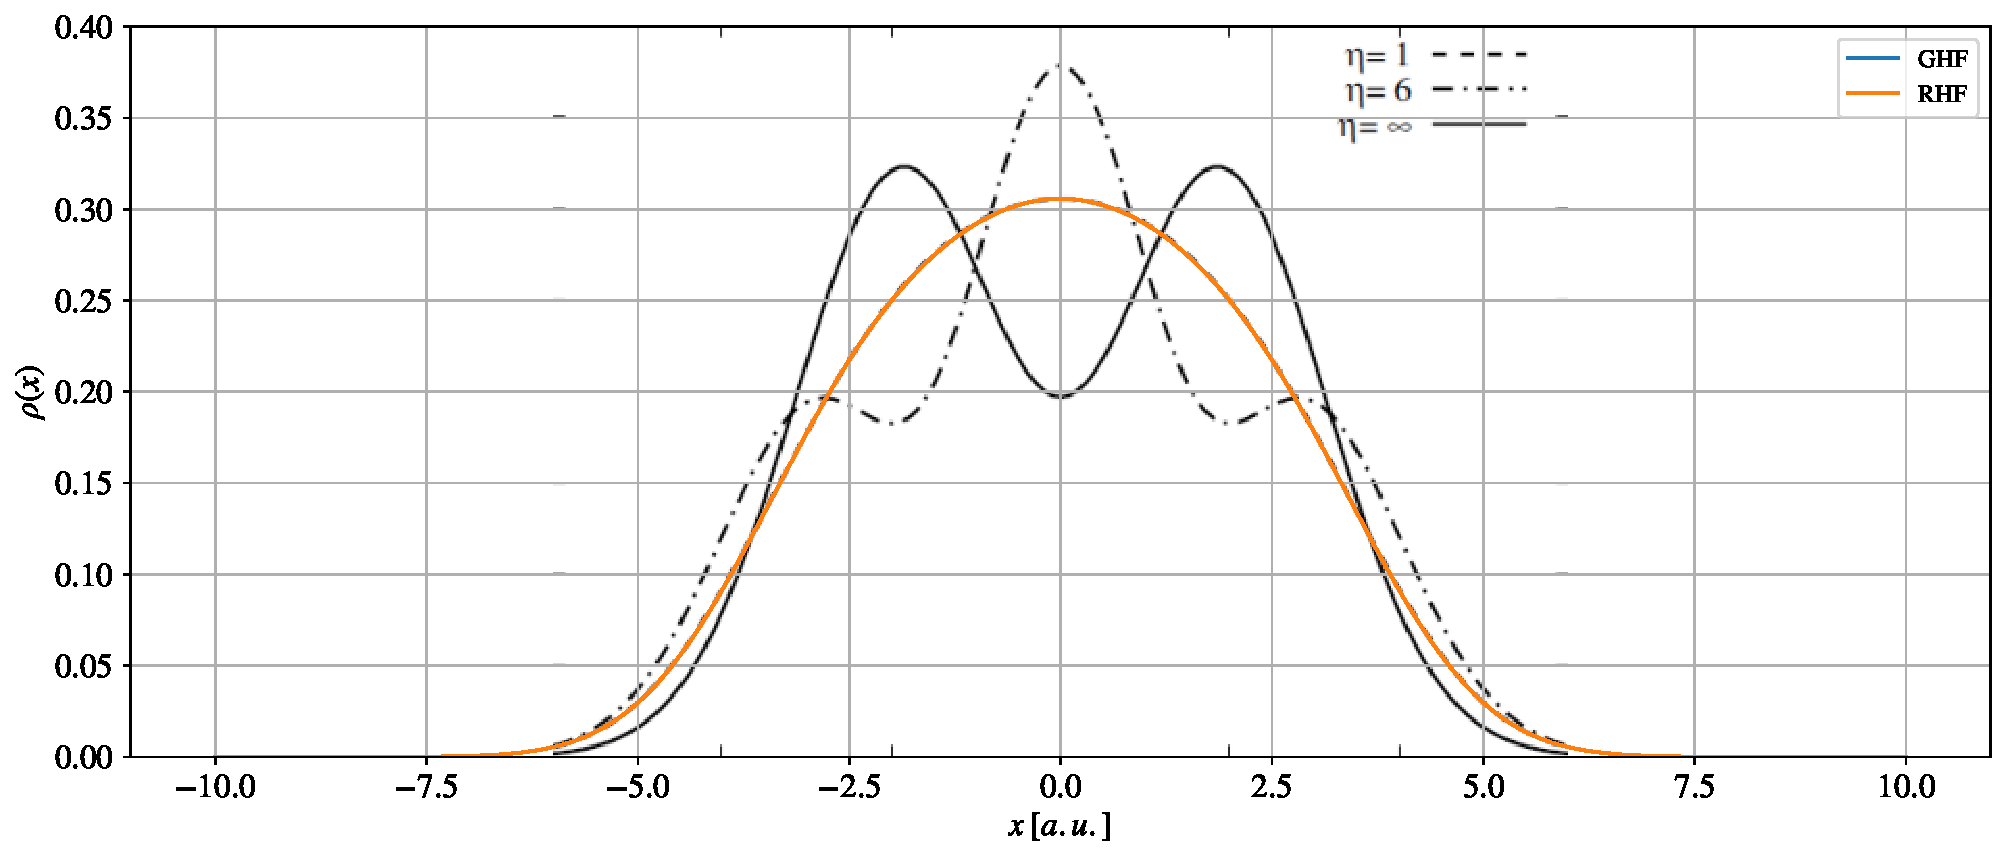
\includegraphics[scale=0.5]{images/onebody_density_comp_article.pdf}
    \caption{Comparison between our estimates for the ground state one-body density and the corresponding result in \cite{Zanghellini_2004} for a system with $\Omega=0.25$ . The obtained curves (which are perfectly overlapped) were produced exploiting the matrix coefficients provided by the convergence of the Ruthaan-Hall equations with $\delta=10^{-6}$, respectively in the general and restricted representation.}
    \label{fig:one_body_density_comp}
\end{figure*}

In order to appreciate possible differences between the general and restricted approach, we launched other simulations with the corresponding time-independent Hartree-Fock solvers, but this time stopping the algorithm after fixed number of $100$ iterations instead of looking at the tolerance $\delta$. In particular, a properly implemented function returned the total energy of the system and the parameter $\Delta$ (see Eq.\,\ref{eq:stop_condition}) evaluated at every step, providing the results shown in Figure \ref{fig:energy_at_every_step} and Figure \ref{fig:delta_at_every_step}.

\begin{figure}[t!]
    \centering
    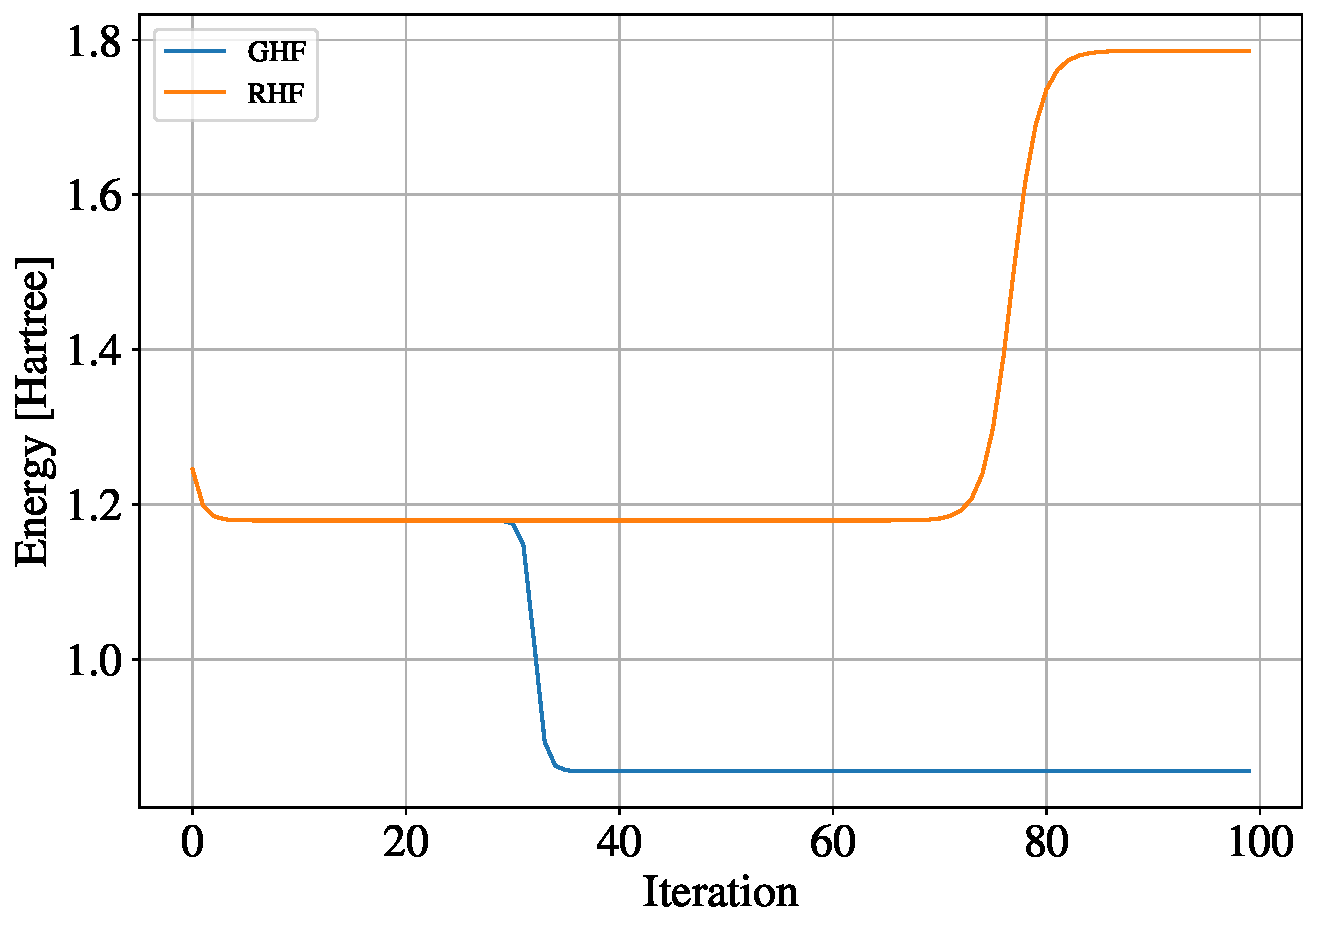
\includegraphics[scale=0.38]{images/energy_at_every_step.pdf}
    \caption{Total energy obtained for each iteration of the time-independent Hartree-Fock solver respectively in the general and restricted representation for a system with $\Omega=0.25$.}
    \label{fig:energy_at_every_step}
\end{figure}

\begin{figure}[t!]
    \centering
    \hspace{-15pt}
    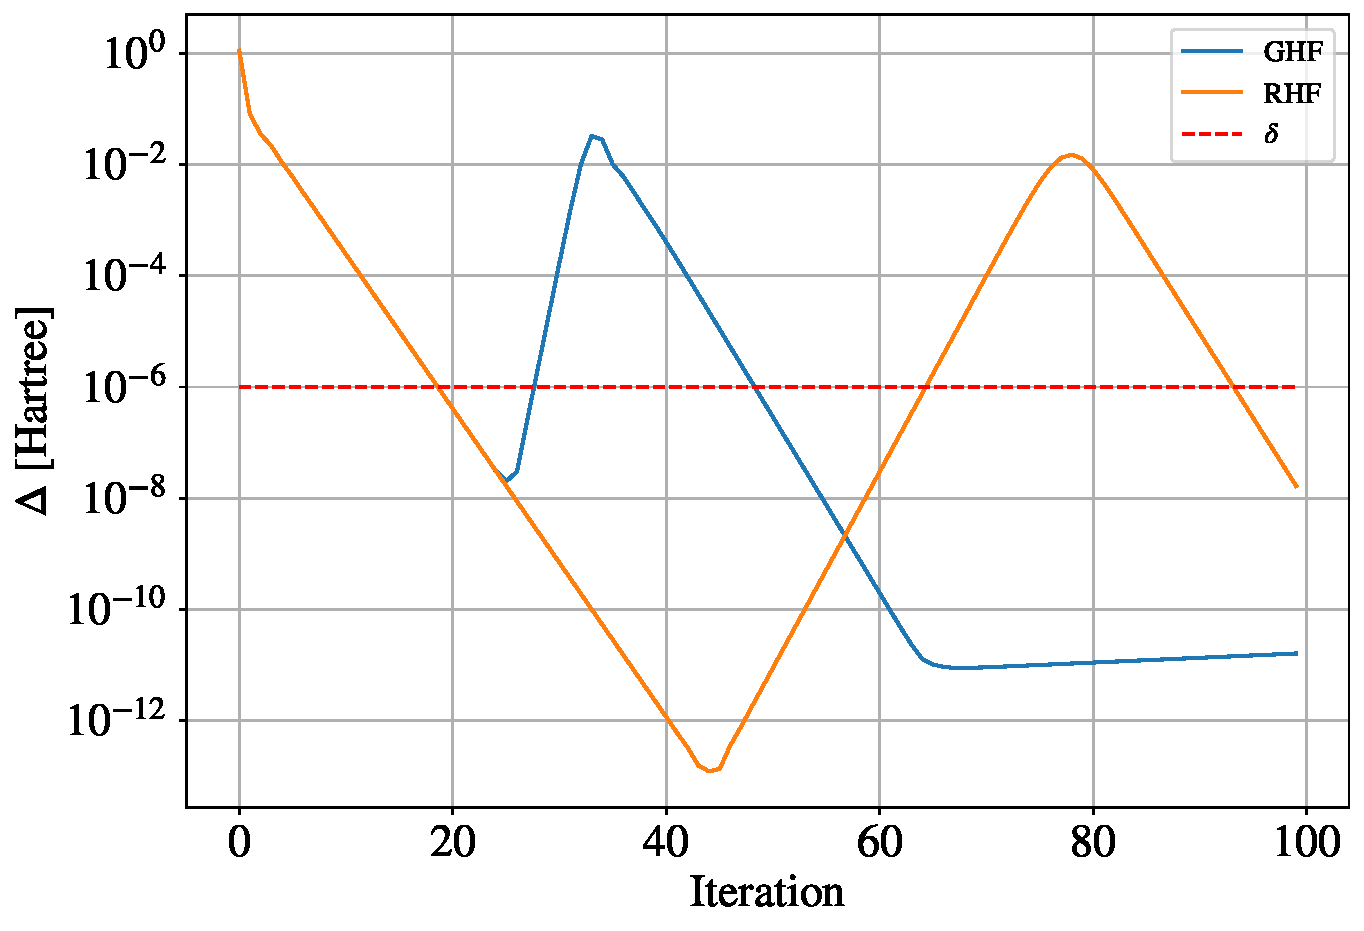
\includegraphics[scale=0.38]{images/delta_at_every_step.pdf}
    \caption{$\Delta$ parameter (see Eq.\,\ref{eq:stop_condition}) evaluated for each iteration of the time-independent Hartree-Fock solver respectively in the general and restricted representation for a system with $\Omega=0.25$. The dashed line represents the threshold value chosen for $\delta$ for the simulations carried out in the context of this project.}
    \label{fig:delta_at_every_step}
\end{figure}



\subsection{TIME-DEPENDENT TREATMENT}
Switching to the time-dependent case, now the comparison with the article by Zanghellini is focused on the overlap between the wavefunction evaluated at $t=0$ and $t\neq 0$, expressed by the parameter $\xi(t)$ defined in Eq.\,\ref{eq:overlap_coeff}. From now on, only the results provided by the general solver will be taken into consideration. In order to reproduce the plots reported in the paper, we exploited the coefficient matrix for the ground state evaluated in the time-independent framework with $\Omega=0.25$ and $\delta=10^{-6}$, using these as a seed for the integrator described in Section \ref{sec:integrator}. We employed a time step $dt=10^{-4}$, allowing for a good compromise between speed and accuracy. Also smaller values for the time step were tested, but they didn't provide any evident improvement in this sense. In addition to the overlap, also the time-evolution of the dipole operator was included in the analysis by inserting into Eq.\,\ref{eq:x_time_dependent_coeff} the coefficient matrix provided by the integrator at each time instant. The results are reported respectively in Figure \ref{fig:overlap_comp_paper} and Figure \ref{fig:dipole_comp}. The procedures described up to now were also applied to other $\omega$ values, the corresponding plots being reported in Figure \ref{fig:overlap_comp_omega} and Figure \ref{fig:dipole_comp} for a comparison with the standard case of $\omega=2$. The one-body density time evolution was also represented together with the behaviour of the one-body potential: these results for the mentioned $\omega$ configurations appear in some animated pictures that one can find \href{https://github.com/Matteo294/FYS4411/tree/main/Project2/code}{here}.  \\

\begin{figure*}[h!]
    \centering
    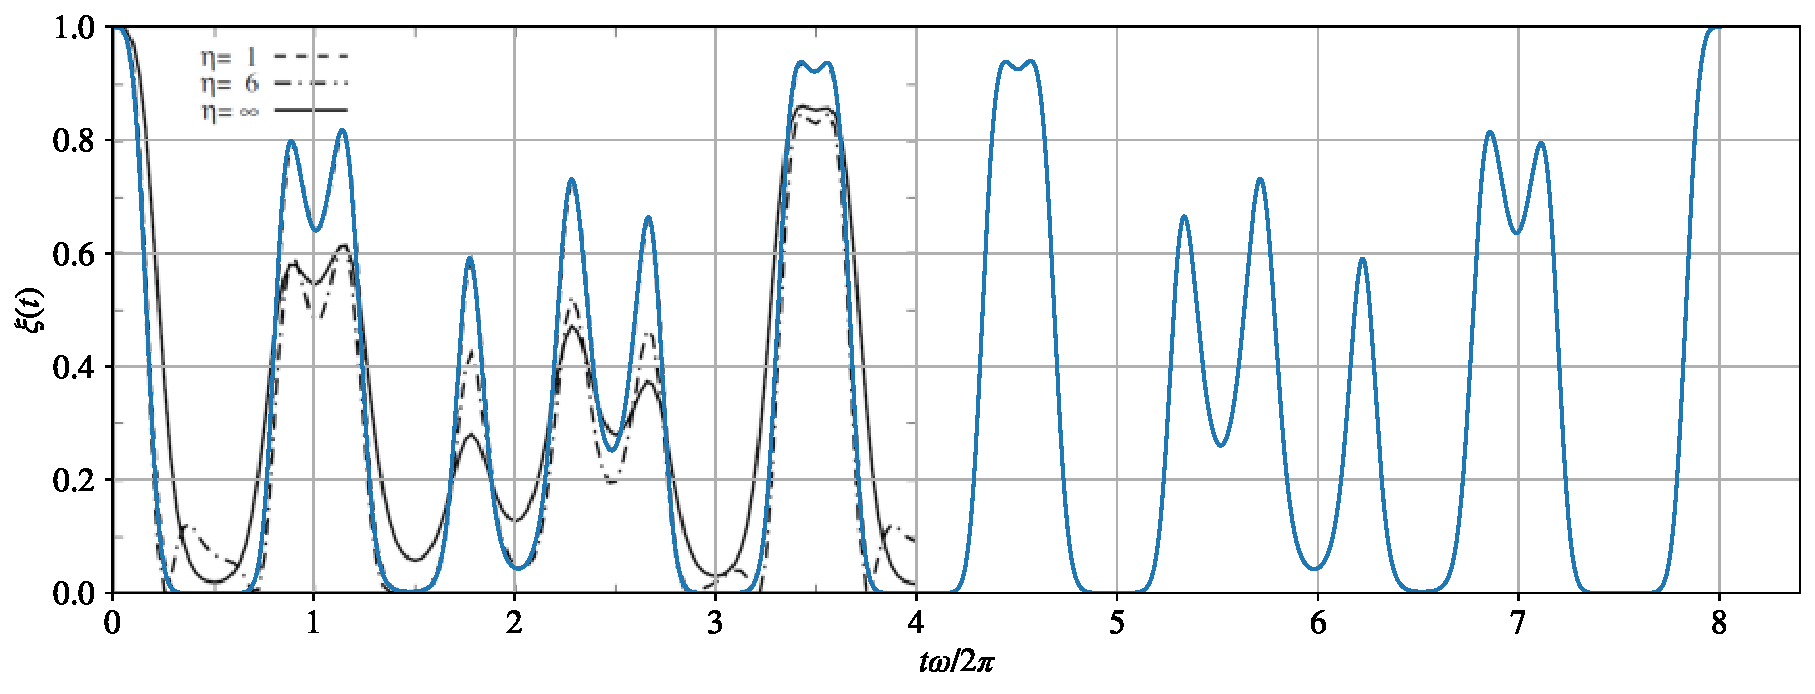
\includegraphics[scale=0.5]{images/overlap_comp_article.pdf}
    \caption{Comparison between the time-evolution of the overlap $\xi(t)$ (see Eq.\,\ref{eq:overlap_coeff}) provided by our code and the corresponding result reported in \cite{Zanghellini_2004} for a system with $\Omega=0.25$ and $\omega=2$, using a time step $\delta t=10^{-4}$. The coefficient matrix used as initial condition for the time evolution corresponds to the resulting one from the convergence of the time-independent solver with $\delta=10^{-6}$. }
    \label{fig:overlap_comp_paper}
\end{figure*}

\begin{figure*}[h!]
    \centering
    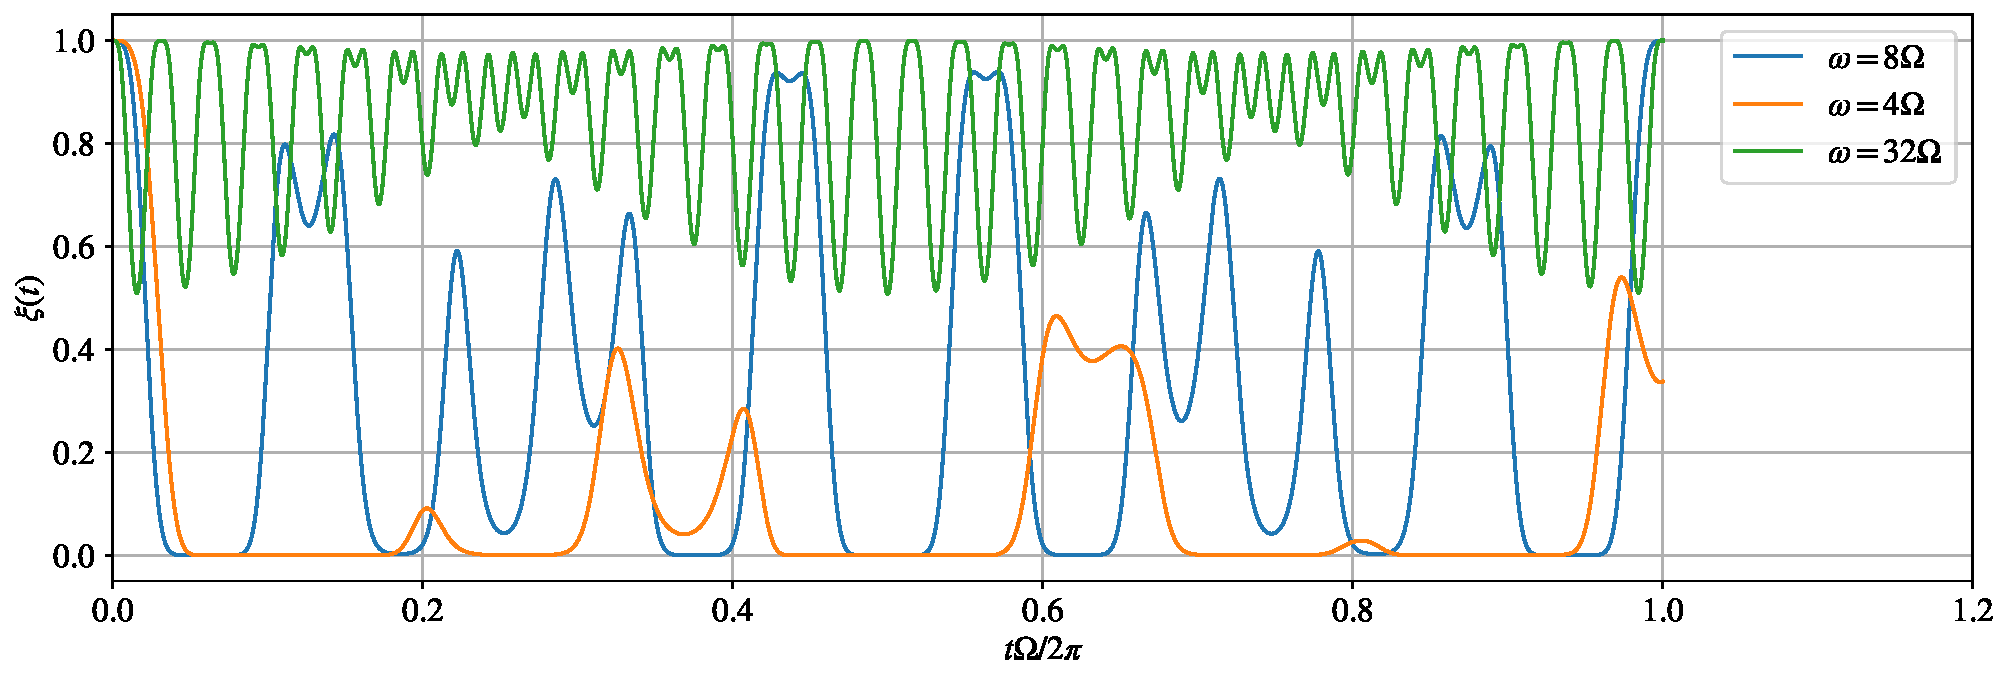
\includegraphics[scale=0.5]{images/overlaps_different_omega.pdf}
    \caption{Comparison between the time-evolution of the overlap $\xi(t)$ (see Eq.\,\ref{eq:overlap_coeff}) provided by our code for $\Omega=0.25$ and different values for $\omega$, using $\delta t = 10^{-4}$. The coefficient matrix used as initial condition for the time evolution corresponds to the resulting one from the convergence of the time-independent solver with $\delta=10^{-6}$.}
    \label{fig:overlap_comp_omega}
\end{figure*}

\begin{figure}[t!]
    \centering
    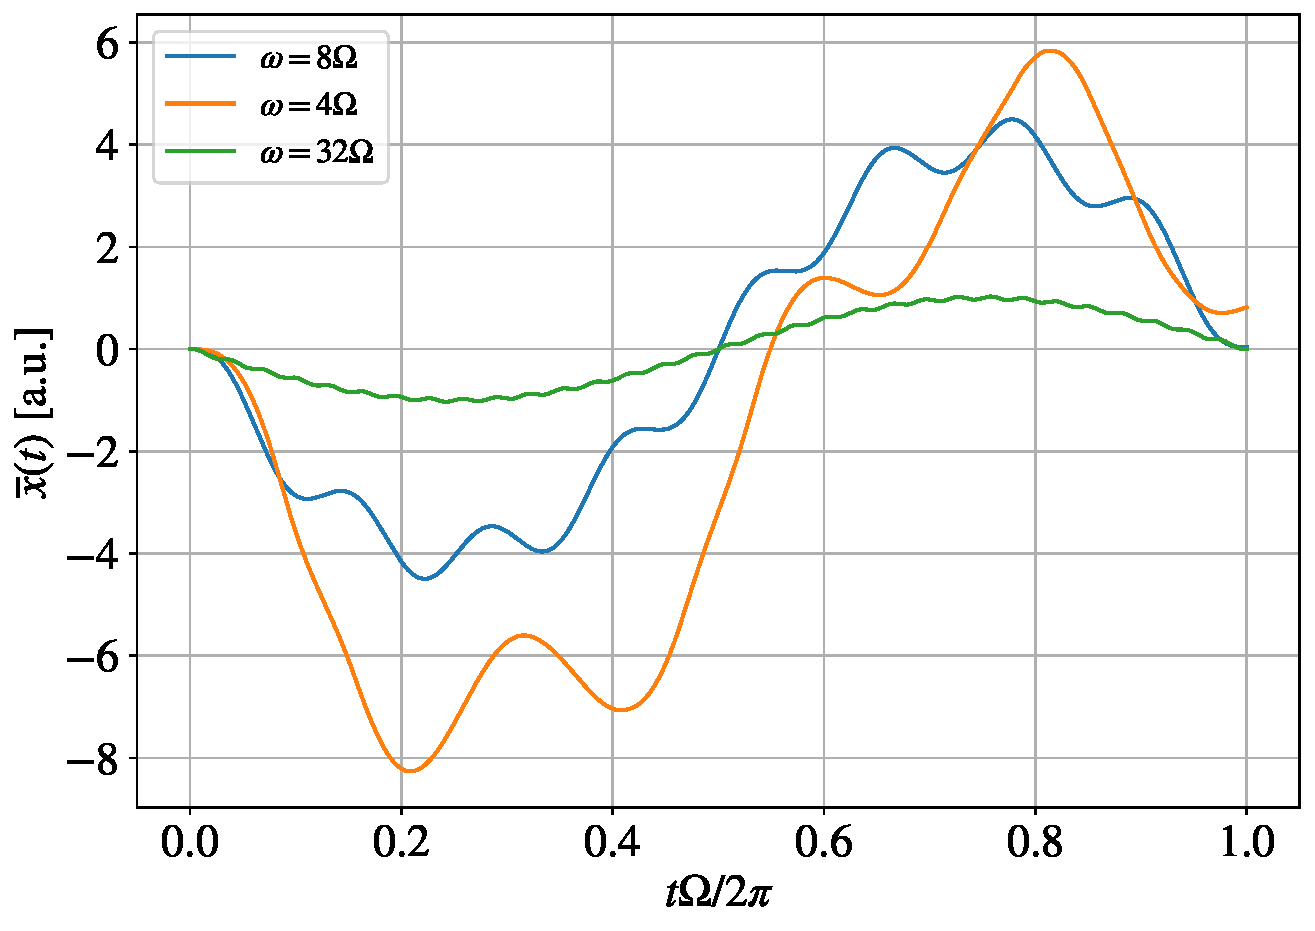
\includegraphics[scale=0.38]{images/dipoles_different_omega.pdf}
    \caption{Time evolution of the dipole operator $\overline{x}(t)$ (see Eq.\,\ref{eq:x_time_dependent_coeff}) for a system with $\Omega=0.25$ and three different $\omega$ values, using $\delta t = 10^{-4}$. The coefficient matrix used as initial condition for the time evolution corresponds to the resulting one from the convergence of the time-independent solver with $\delta=10^{-6}$.}
    \label{fig:dipole_comp}
\end{figure}


Finally, we report the results obtained in the context of the Fourier analysis described in Section \ref{sec:fourier_analysis}. For this purpose, we launched a time-evolution of the system with the laser source active for a time $T=10\pi$, then the simulation proceeded with the laser turned off until $T_f = 100\pi$. For the simulation we adopted $dt=10^{-4}$, evaluating at each instant the parameters $\xi_T(t)$ and $\overline{x}(t)$ defined in Eq.\,\ref{eq:overlap_T_coeff} and Eq.\,\ref{eq:x_time_dependent_coeff}. The points of these curves obtained for $t\in (T,T_f)$ were then processed with the FFT algorithm. In particular, the procedure described up to now was repeated for three different values of $\Omega$ and $\omega$, in order to find a possible correlation between them and the frequency components appearing in the spectrum. For each run with different $\Omega$ we exploited as seed the corresponding ground-state coefficient matrix provided by the general Hartree-Fock solver with $\delta=10^{-6}$.

For all the considered simulations, the same values for cited above for $T$ and $T_f$ were used. The curves for $\overline{x}(t)$ and $\xi_T(t)$ reported in Figure \ref{fig:laser_on_off} and Figure \ref{fig:overlap_T} are referred to $\Omega=0.25$ and $\omega=8\Omega=2$, while the spectra appearing in Figure \ref{fig:fourier_spectra_x} and Figure \ref{fig:fourier_spectra_xi} correspond to the configurations reported in the respective legends. The reliability of the implemented code was enforced by the fact that the energy of the system remained constant after the laser source was switched off.

\afterpage{
\begin{figure}[t!]
    \centering
    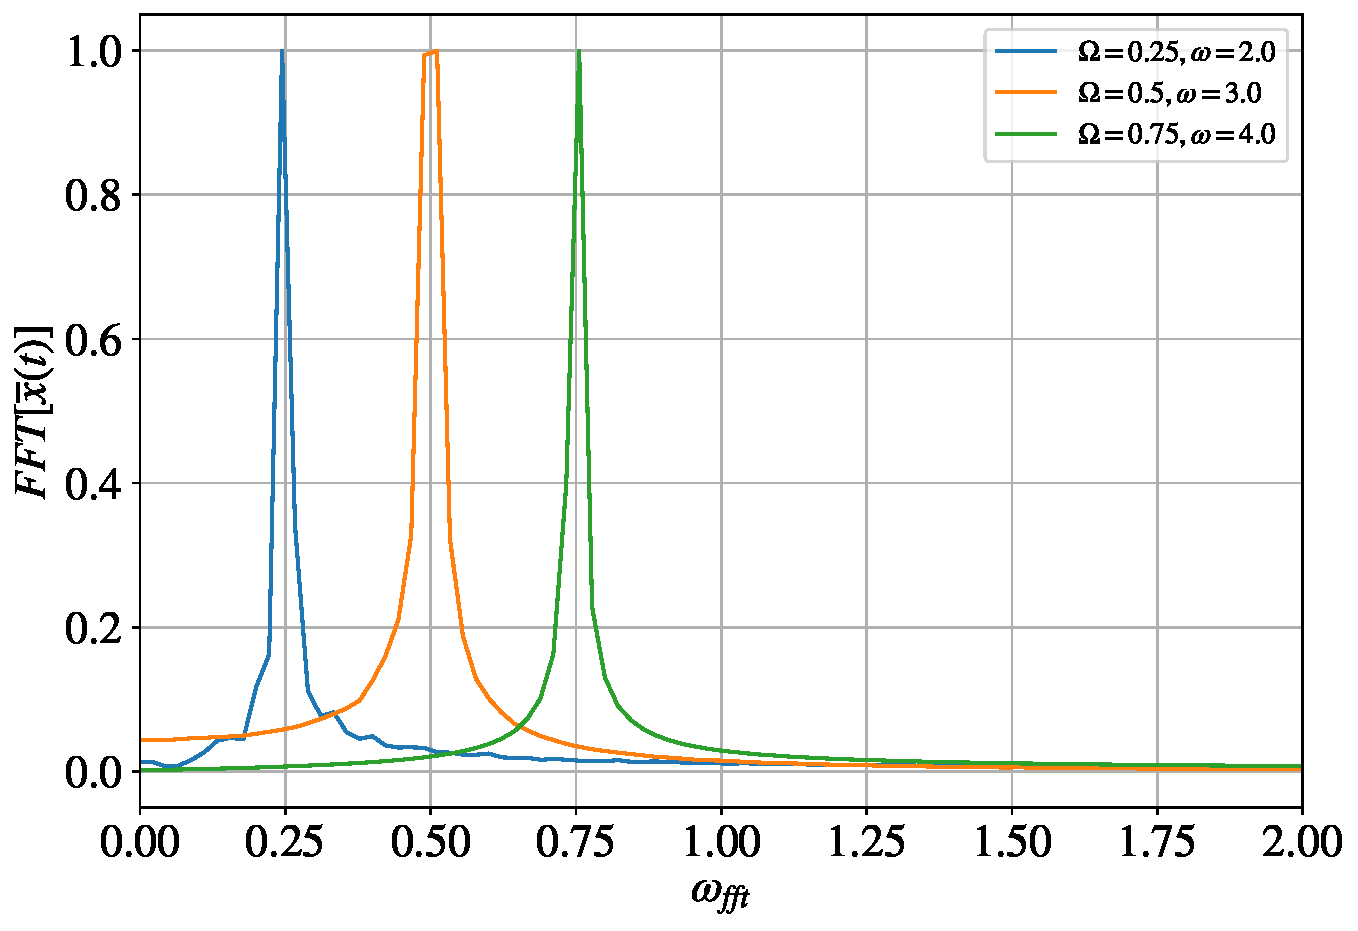
\includegraphics[scale=0.38]{images/spectra_x_diff_omegas.pdf}
    \caption{Normalized Fourier spectra of the signal $\overline{x}(t)$ with $t \in (T,T_f)$ for three different combinations of $\Omega$ and $\omega$, using $\delta t = 10^{-4}$. In each time-evolution the laser source was left active for $t \in (0, T)$ and then switched off for $t\in(T,T_f)$, being $T=10\pi$ and $T_f=100\pi$. The coefficient matrix used as initial condition for the time evolution corresponds to the resulting one from the convergence of the time-independent solver with $\delta=10^{-6}$.}
    \label{fig:fourier_spectra_x}
\end{figure}
}
\afterpage{
\begin{figure}[t!]
    \centering
    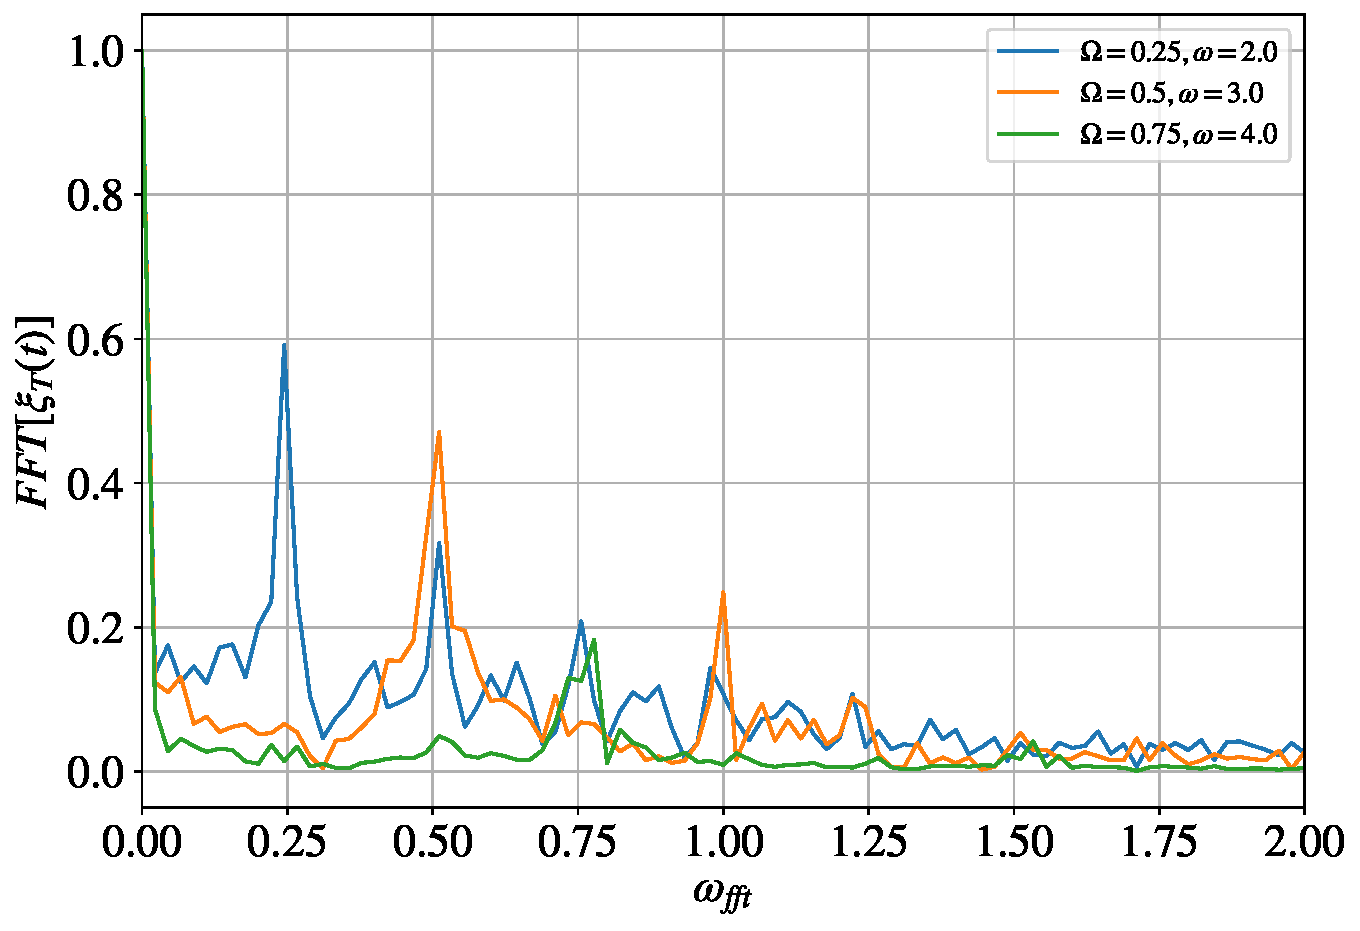
\includegraphics[scale=0.38]{images/spectra_xi_diff_omegas.pdf}
    \caption{Normalized Fourier spectra of the signal $\xi_T(t)$ with $t \in (T,T_f)$ for three different combinations of $\Omega$ and $\omega$, using $\delta t = 10^{-4}$. In each time-evolution the laser source was left active for $t \in (0, T)$ and then switched off for $t\in(T,T_f)$, being $T=10\pi$ and $T_f=100\pi$. The coefficient matrix used as initial condition for the time evolution corresponds to the resulting one from the convergence of the time-independent solver with $\delta=10^{-6}$.}
    \label{fig:fourier_spectra_xi}
\end{figure}
}

\begin{figure*}[h!]
    \centering
    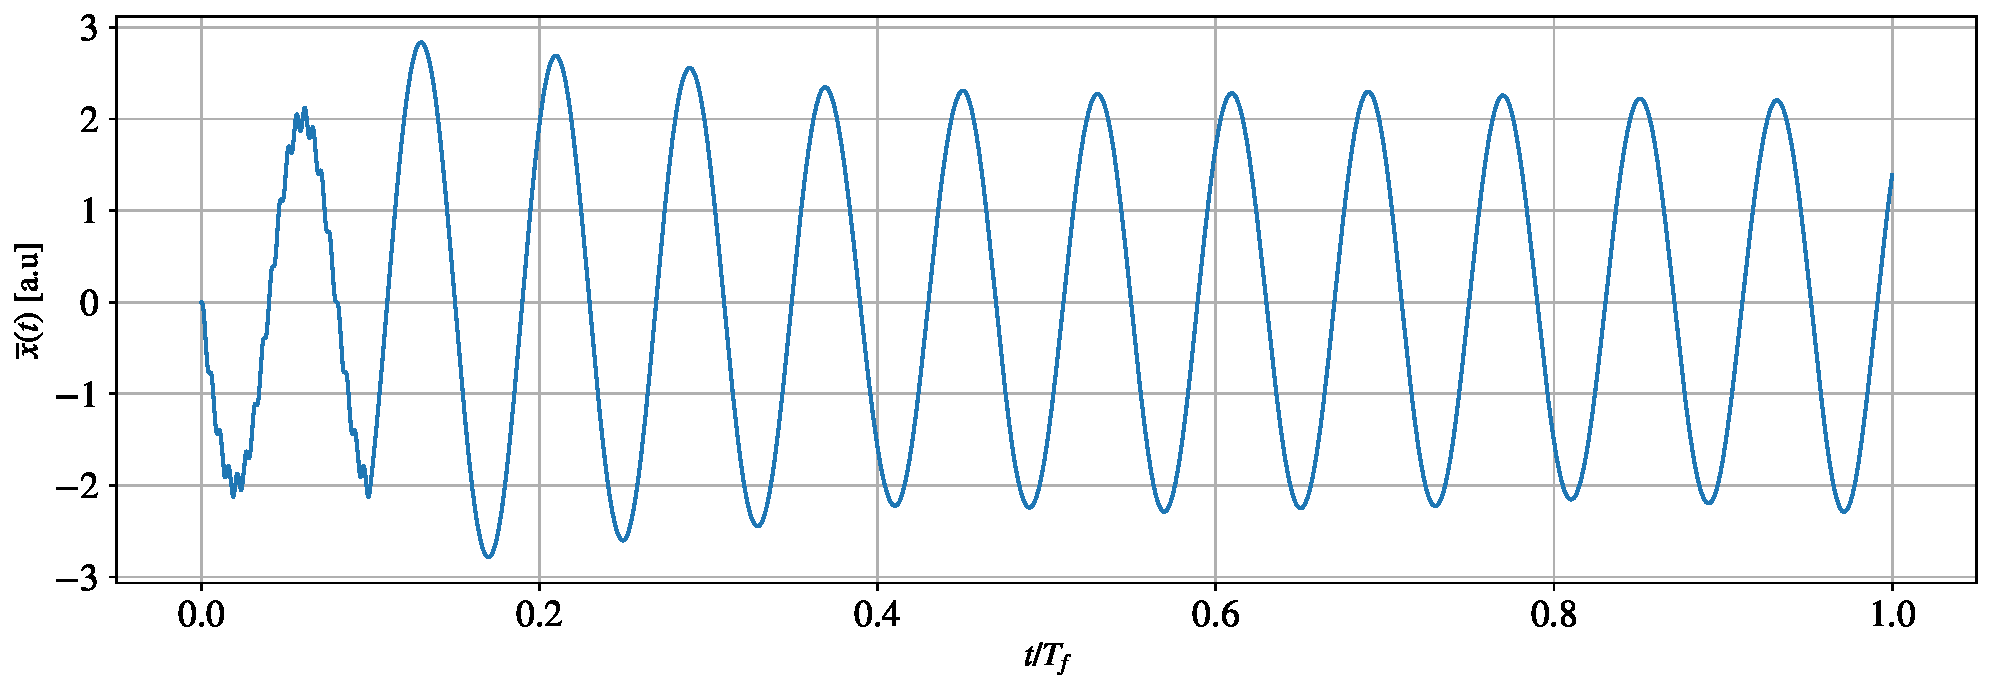
\includegraphics[scale=0.5]{images/dipole_laser_ONOFF.pdf}
    \caption{Time evolution of $\overline{x}(t)$ (see Eq.\,\ref{eq:x_time_dependent_coeff}) with laser source active for $t\in(0, 10 \pi)$ and then switched off up to $T_f=100\pi$. The coefficient matrix used as initial condition for the time evolution corresponds to the resulting one from the convergence of the time-independent solver with $\delta=10^{-6}$. Plotted results are referred to a system with $\Omega=0.25$ and $\omega=2$ and the time step used is $\delta t = 10^{-4}$. }
    \label{fig:laser_on_off}
\end{figure*}

\begin{figure*}[h!]
    \centering
    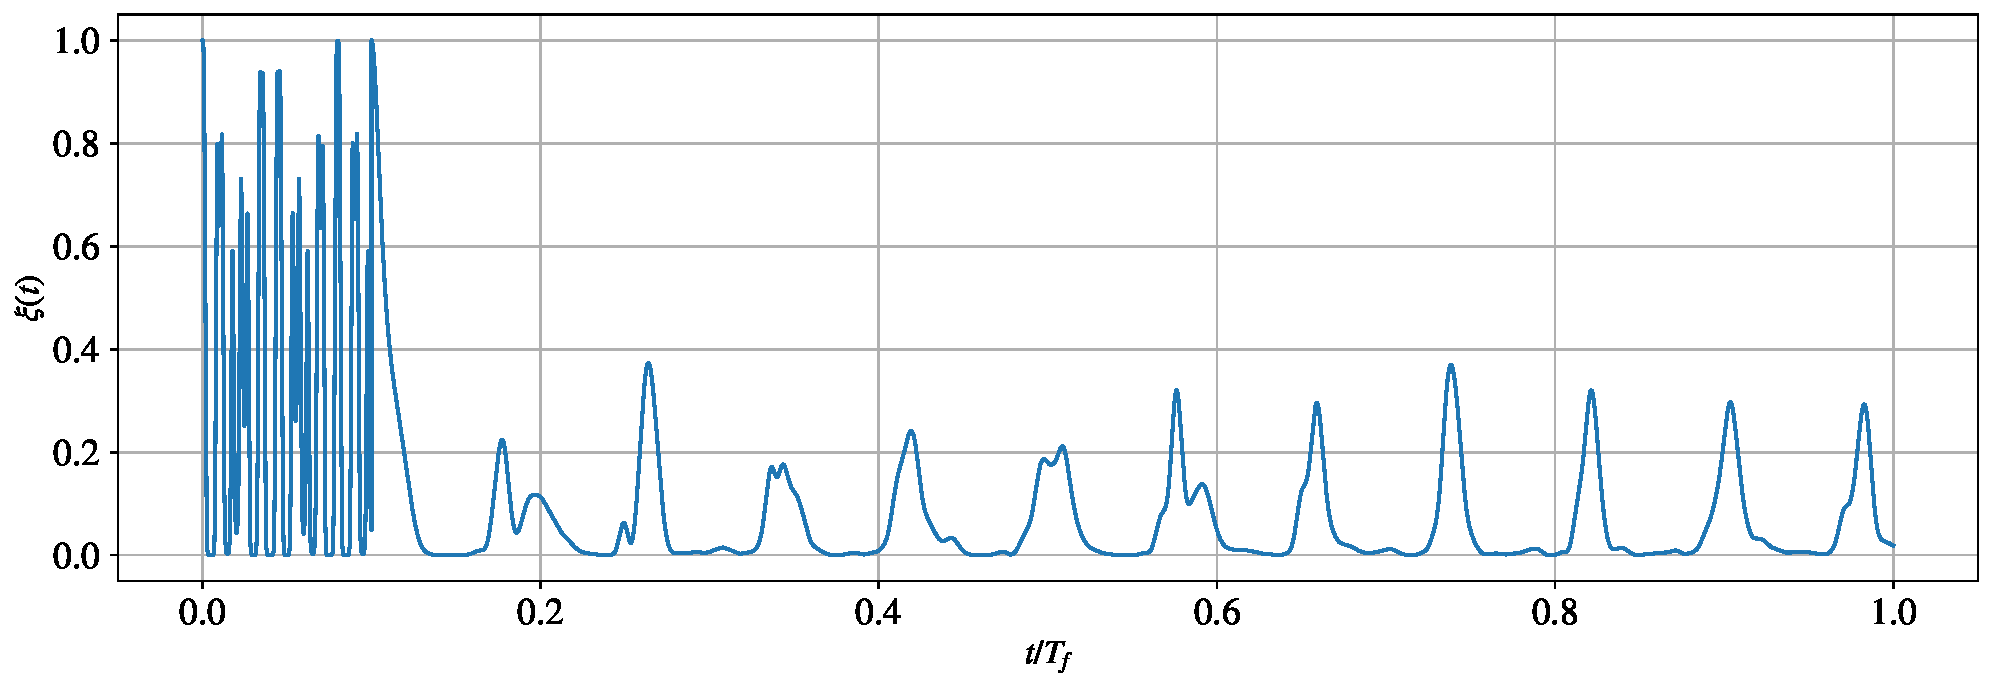
\includegraphics[scale=0.5]{images/overlap_laser_ONOFF.pdf}
    \caption{Time evolution of $\xi (t)=\vert \braket{\Psi(t)}{\Psi(0)} \vert^2$ for $t/T_f<0.1$ and $\xi_T (t)=\vert \braket{\Psi(t)}{\Psi(T)} \vert^2$ for $t/T_f>0.1$ with laser source active for $t\in(0, 10 \pi)$ and then switched off up to $T_f=100\pi$. The coefficient matrix used as initial condition for the time evolution corresponds to the resulting one from the convergence of the time-independent solver with $\delta=10^{-6}$. Plotted results are referred to a system with $\Omega=0.25$ and $\omega=2$  and the time step used is $\delta t = 10^{-4}$. }
    \label{fig:overlap_T}
\end{figure*}



\section{DISCUSSION ABOUT THE RESULTS}
\label{sec:discussion}
Considering at a first stage the time-independent Hartree-Fock solver, we can see that our code provided us with a faithful reproduction of the results contained in the paper from Zangellini et al. Both the general and restricted representation implemented on our side revealed to be effective in this task: in fact the total energy values appearing in Table \ref{tab:E_x_comp_article} and the one-body density shown in Eq.\,\ref{fig:one_body_density_comp} perfectly match the estimated provided in the article. In addition, the two expected values for the position operator appear to be on the order of $10^{-10}$ in magnitude, thus reasonably compatible with the null value. Furthermore, as expected, we observe that the integral of the one-body densities gives us the number of particles. These result were not reported in the article, but still they are consistent with the symmetrical shape of the one body density and its expected normalization. These procedures acted also as a verification of the correct implementation of the various functions, giving us a high confidence in using the ground state coefficient matrix as a seed for the subsequently performed time evolution.\\

Further analysis of the convergence properties of the general and restricted Hartree-Fock solvers revealed some interesting aspects. Considering the results for the energy evaluated at every iteration reported in Figure \ref{fig:energy_at_every_step}, we can notice a first plateau reached after few steps by both the systems, followed by a split of the two curves. The apparatus described by the general representation explores a region of lower energy, converging to a more stable state after some iterations. This is proved also by the behaviour of the corresponding $\Delta$ parameter reported in Figure \ref{fig:delta_at_every_step}: here we can appreciate the fact that the smallest $\Delta$ values appear in correspondence of the second plateau in the energy diagram. A little grow around the $70$-th iteration occurs, this probably being a symptom of some instability of the algorithm. However, it is worth noticing that the convergence to a lower energy state follows as a consequence of the spin mixing allowed in the general representation: in this context, the system will converge to the energetically most favourable state, which cannot be explored by the other system, since the restricted implementation does not allow for spin mixing. 

In this second case, the adopted solver reaches better stability within fewer iterations, as clearly seen also in Figure \ref{fig:delta_at_every_step}. We also notice an inversion of the slope for $\Delta$ around the $40$-th iteration, corresponding then to an inversion in the energy curve as the number of steps increases. These unexpected behaviours can reasonably be symptoms of instabilities of the algorithm, since the variational principle that drove the derivation of the Hartree-Fock theory seems to be even no more satisfied. 

Concluding the discussion about the time-independent solver, we can say that the imposition of a lower tolerance in the general solver would have led the convergence to a lower energy state. However, we still opted to keep the tolerance to $\delta=10^{-6}$, in order to be able to make some comparisons with the content of the article by Zanghellini et al. \\


Switching then to the time domain, the overlap curve presented in Figure \ref{fig:overlap_comp_paper} almost perfectly matches the one presented in the article: this being a further confirmation of the goodness of the implemented code also when time enters into play. Plotting the time evolution of the overlap for a long time allowed us to appreciate the almost perfect symmetry of the $\xi(t)$ curve, which results to be specular with respect to the vertical line passing in $t\omega/2\pi=4$. In particular, after a whole period of oscillation of $2\pi/\Omega$ inside the harmonic potential, we can see that the system returns very close to its original state. The frequency with which this occurs is, in our case, the same as the frequency of the harmonic oscillator in which the electrons are confined. However, a prolonged plot showed that after a few periods the symmetry of the curve was lost: we didn't analyze in depth the reasons behind this, which could however consist in the finite precision of the integrator or more simply in a natural deviation of the system from the symmetrical behaviour. \\ 

Other tests performed with different values of $\omega$ revealed that this symmetric behaviour occurs for small $t$ independently from the chosen $\omega$, under the condition that $\omega \gtrsim 8\Omega$. This can possibly be explained by analyzing the effect brought in by the laser source: the time-dependent potential introduced in Eq.\,\ref{eq:hamiltonian_t_dip} indeed acts on the system by modifying at each time instant the position and the depth of the minimum in the harmonic oscillator potential. The higher is the frequency of the laser source, the harder is for the system to adapt rapidly to the changes induced in the single particle potential before an oscillation in the laser term is actually completed. The system will then spend much time close to the initial state, as shown also in Figure \ref{fig:overlap_comp_omega}: here one appreciates the fact that the overlap curve assumes on average higher values in correspondence of large $\omega$.  On the contrary, when the values of $\omega$ and $\Omega$ are comparable, the effects introduced by the laser source are much more evident since the system gets close to a resonant behaviour. In this last case, the symmetry of the curve is broken. For a better visualization of these concepts, please refer to the animated pictures reported \href{https://github.com/Matteo294/FYS4411/tree/main/Project2/code}{here}.

The considerations about the symmetry described up to now are very evident also in Figure \ref{fig:dipole_comp}. The oscillations in the curves for $\omega=8\Omega$ and $\omega=32\Omega$ follow a sinusoidal behaviour with a frequency $\Omega$, while the little wiggles are attributable to the component provided by the laser source with a frequency $\omega$. As this last parameter increases in value, the curve appears to be more an more similar to a pure sinusoidal wave at frequency $\Omega$, while evident early breaks in the symmetry induced by the resonant behaviour appears for small $\omega$ values. \\


Exploiting again the time dependent solver, we performed another evolution of the system with the laser kept in operation for a limited period and then switching it off for the rest of the simulation. The curve obtained for $\overline{x}(t)$ reported in Figure \ref{fig:laser_on_off} shows the already described behaviour for $t<T$, then becoming much more similar to a pure sinusoidal wave when the laser is switched off. The same behaviour also occurs for other combinations of $\Omega$ and $\omega$ and appears to be evident in the frequency spectra presented in Figure \ref{fig:fourier_spectra_x}. Here the main peaks should appear in correspondence of the transition energy values between the various excited states of the considered time-independent system, but, as we see, just one sharp line appears. We could suppose that the absence of other lines is due to the form of Eq.\,\ref{eq:transition_energies}: here each complex exponential oscillating at frequency $\omega_{ij}$ is multiplied by the corresponding $\bracketOP{\Psi_i}{\Psi_j}{\hat{x}}$. It may occur that this expected value is null for certain combinations of $i$ and $j$, annihilating also the corresponding contributions in the spectrum for the frequency of interest in this context. \\

Finally, the curve for $\xi_T(t)$ presented in Figure \ref{fig:overlap_T} is not so informative about the transition frequencies, thus for a better comprehension we must recur to the actual spectra presented in Figure \ref{fig:fourier_spectra_xi}. Here many more frequencies appear in the spectrum, the majority of them probably caused by some noise in the overlap curves induced by the discrete time integration. However, among them it is possible to distinguish some higher peaks: further analysis may be performed to better analyze the origin of these peaks, especially for what concerns their relation with the frequency $\Omega$. Indeed, they appear to be approximately equally spaced of a factor $\Omega$, suggesting some strong link with the typical spectrum of an harmonic oscillator. Moreover, the intensity of the peaks goes diminishing for increasing values of $\omega_{fft}$, symptom of the fact that the state in which we leave the system after the laser has been switched off is given by a superposition of different states, with major contribution given by those possessing lower energy. 

% In the first part of the evolution, both the particles are forced to follow the minimum of the harmonic oscillator potential, which moves at every time instant under the effect brought in by the laser source. Later in time, the harmonic hole returns to be steadily centered in $x=0$ and the two electrons are then free to oscillate into the hole itself, giving rise to the sinusoidal part of the curve for $t>T$. In this last part of the evolution, the two electrons' behaviour becomes comparable with a classical one, with the mentioned oscillations that we are used to see associated to a classical particle inserted in a harmonic potential.

% This similarity with the classical behaviour appears even more evident when we come then to the analysis of the frequency components generating the signal for $t>T$. We can notice from Figure \ref{fig:fourier_spectra} that the main peak is given in each case by the frequency associated to the harmonic oscillator potential and no correlations with the value of $\omega$ appear. 

\section{POSSIBLE FURTHER IMPROVEMENTS}
\label{sec:improvements}
As previously said, the restricted solver has been employed only for a comparison with the corresponding results for the ground state coming associated to the general representation. The restricted solver has not been used in the time-dependent context, thus further integrations and testings of the code can be performed. 

All the results presented above for the time-dependent system would require a more detailed analysis and further tests: a longer time for the simulations is recommended, and more combinations of $\Omega$ and $\omega$ can be implemented, varying also the time spent with the laser source in operation.

Finally, the mentioned analysis can be applied also to the time-evolved version of the ground state provided by the general solver for lower values of tolerance. All the procedures could be testing also varying the number of eigenstates of the harmonic oscillator that we employ for the expansion of the single particle states.

\section{CONCLUSIONS}
\label{sec:conclusions}
Both the general and restricted implementations allowed us to reproduce the results for the ground state energy and one-body density reported in \cite{Zanghellini_2004}. The analysis of the convergence properties for the two spin representations revealed that the general solver allowed the system to explore regions even lower in energy, but this would have prevented us from further constructive comparisons with the results obtained by Zanghellini et al. \\

The so-obtained matrix coefficient generated after the convergence of the general solver was then used as seed for all the further time evolutions. In particular, the chosen integrator allowed us to reproduce again the results presented in \cite{Zanghellini_2004} for what concerns the overlap integral, enforcing the reliability of our code. Other simulations performed also with different values of $\omega$ revealed that both the curves $\xi(t)$ and $\overline{x}(t)$ show an approximate periodicity given by $2\pi/\Omega$, which appears more evident only for small $t$ and $\Omega \gtrsim 8\omega$. In particular, the higher the frequency of the laser with respect to the one associated to the harmonic potential, the longer is the time spent by the system near to the initial ground state. This behaviour may be symptom of the fact that the system shows a certain inertia which prevents it from fast adaptations to the changes in the potential induced by the laser field, especially when those changes occur at high frequency. Lower values of $\omega$ put the system closer to a resonant behaviour, thus letting the system to adapt to the induced changes with the consequent early breaking of the mentioned symmetries. \\

The time-evolution with the laser source first active and then switched off was then performed. The spectrum associated to $\xi_T(t)$ was populated by many transition energy values: their spacing reminds to the typical spectrum associated to a system trapped in a harmonic oscillator potential, but further analysis should be performed in this context. The Fourier analysis of the curve $\overline{x}(t)$ for $t>T$ revealed that not all the expected frequencies appeared in the plot: this may be attributable to the annihilation of some components given by a null value of $\bracketOP{\Psi_i}{\Psi_j}{\hat{x}}$. 

Many more configurations could be tested for each of the mentioned points, testing also different values for many parameters.





\section*{LINK TO GITHUB REPOSITORY}
\centerline{\href{https://github.com/Matteo294/FYS4411}{\texttt{https://github.com/Matteo294/FYS4411}}}


% \newpage
% \section{Derivation of the Hartree-Fock method}
% In this section we want to provide a derivation of the Hartree-Fock equations mainly referring to \cite{bransden}, in the special case of the ground state of a system populated by $N$ electrons. \\
The hamiltonian that describes such a system is assumed to be 
\begin{equation*}
    \mathcal{H} = \mathcal{H}_1 + \mathcal{H}_2
\end{equation*}
where $\mathcal{H}_1$ is the single particle hamiltonian (or one body hamiltonian)
\begin{equation*}
    \mathcal{H}_1 = \sum_{i=1}^N h_i = \sum_{i=1}^N -\frac{1}{2}\nabla_{\ve{r}_i}^2 + V(r_i)
\end{equation*}
and $\mathcal{H}_2$ is the interaction term
\begin{equation*}
    \mathcal{H}_2 = \sum_{i<j,j=1}^N v(r_i, r_j)
\end{equation*}
Since we are dealing with a system of fermions, the wavefunction describing the ground state of the system $\Phi^*(q_1, \dots, q_N)$ must be antisymmetric under the action of the permutation operator $P$ so that
\begin{gather*}
    P_{ij} \Phi^*(q_1, \dots,q_i, \dots, q_j, \dots, q_N) = \\
    = \Phi^*(q_1, \dots, q_j, \dots, q_i, \dots, q_N) = \\ 
    = - \Phi^*(q_1, \dots, q_i, \dots, q_j, \dots, q_N) 
\end{gather*}
The central idea of the method consists in assuming that the ground state wavefunction $\Phi^*(q) \equiv \Phi^*(q_1, \dots, q_N)$ can be approximated by a Slater determinant of single particle wavefunctions
\begin{equation*}
    \Phi^*(q) \approx \Phi(q) \equiv \frac{1}{\sqrt{N!}} \ \begin{vmatrix} \phi_{\alpha}(q_1) \ \phi_{\beta}(q_1) \ \dots \ \phi_{\nu}(q_1) \\ 
    \phi_{\alpha}(q_2) \ \phi_{\beta}(q_2) \ \dots \ \phi_{\nu}(q_2) \\
    \dots \\
    \dots \\
    \dots \\
    \phi_{\alpha}(q_N) \ \phi_{\beta}(q_N) \ \dots \ \phi_{\nu}(q_N)
    \end{vmatrix}
\end{equation*}
and then make use of the variational principle
\begin{equation}
    \bracketOP{\Phi^*}{\Phi^*}{H} = \mathbb{E}[\Phi^*] \leq \mathbb{E}[\Phi] = \bracketOP{\Phi}{\Phi}{H}
    \label{eq:en_ground_slater_1}
\end{equation}
to find the single particle function $\phi_{\alpha}, \dots \phi_{\nu}$ that minimize the expectation value of the energy $\mathbb{E}[\Phi]$. \\
Each of the subscripts $\alpha, \beta, \dots, \nu$ used in the definition of $\Phi$ refers to a particular set of quantum numbers $(n, l, m_l, m_s)$ so that the notation $\phi_{\mu}(q_i)$ stands for the single electron orbital identified by the set of quantum numbers $\mu = (n^\mu, l^\mu, m_l^\mu, m_s^\mu)$ evaluated in the position of the particle $i$. \\
We also require that ${\phi_{\mu}(q_i)}$ is an orthonormal basis set, so that $\langle \phi_{\mu}|\phi_{\lambda}\rangle =\delta_{\lambda, \mu} $ .\\
The approximated wavefunction can be rewritten by making use of the antisymmetrizer operator $\mathcal{A}$:\footnote{The definition and all the properties of the antisymmetrizer operator can be found at \href{https://en.wikipedia.org/wiki/Antisymmetrizer}{https://en.wikipedia.org/wiki/Antisymmetrizer}}

\begin{align*}
    \Phi(q) &= \frac{1}{\sqrt{N!}}\bigg(\sum_P (-1)^P \hat{P} \bigg) \Phi_H(q) \\
     &= \sqrt{N!} \, \mathcal{A} \, \Phi_H(q)
\end{align*}
where $\hat{P}$ indicates the permutation operator and $\Phi_H(q)$ is:
\begin{equation*}
    \Phi_H(q) = \phi_\alpha(q_1) \, \phi_\beta(q_2) \, \dots \, \phi_\nu(q_N)  
\end{equation*}
Using the variational principle one can estimate the energy of the ground state with the initial guess on $\Phi$.
Starting from equation \ref{eq:en_ground_slater_1}
\begin{align*}
    \mathbb{E}[\Phi^*] &= \bracketOP{\Phi^*}{\Phi^*}{H} \\
    &= \bracketOP{\Phi^*}{\Phi^*}{H_1} + \bracketOP{\Phi^*}{\Phi^*}{H_2}
\end{align*}
Let us study the $H_1$ term. Exploiting the fact that $[\mathcal{A}, H_1]=0$, one gets 
\begin{align*}
    \bracketOP{\Phi^*}{\Phi^*}{H_1} &= N! \bracketOP{\Phi_H}{\Phi_H}{\mathcal{A}H_1\mathcal{A}} \\
    &= N! \bracketOP{\Phi_H}{\Phi_H}{H_1\mathcal{A}^2} \\
    &= N! \bracketOP{\Phi_H}{\Phi_H}{H_1\mathcal{A}} \\
    &= \sum_{i=1}^N \sum_P (-1)^P \bracketOP{\Phi_H}{\Phi_H}{h_i\hat{P}} \\
\end{align*}
In the last sum over the possible permutations, the only term that survives  is obtained when the permutation operator coincides with the identity operator. This happens because we choose an orthonormal basis set for $\psi_{\mu}(q)$, this yields to: 
\begin{align*}
    &= \sum_{i=1}^N  \bracketOP{\Phi_H}{\Phi_H}{h_i}
\end{align*}
Now one can rewrite the summation running over the N individual quantum states rather than particles. 
This notation will be helpful in the derivation. 
\begin{align*}
    &= \sum_{\lambda} \bracketOP{\phi_\lambda}{\phi_\lambda}{h_i}\\
    &= \sum_{\lambda} I_\lambda
\end{align*}
We indicated with $I_{\lambda}$ the average value of the individual hamiltonian $h_i$ relative to the spin orbital $\phi_{\lambda}$.
Now focusing on the $H_2$ interaction term, exploiting the fact that $[\mathcal{A}, H_2]=0$
\begin{align*}
    \bracketOP{\Phi}{\Phi}{H_2} &= N! \bracketOP{\Phi_H}{\Phi_H}{\mathcal{A}H_2 \mathcal{A}} \\
    &= N! \bracketOP{\Phi_H}{\Phi_H}{H_2 \mathcal{A}} \\
    &= \sum_P (-1)^P  \bracketOP{\Phi_H}{\Phi_H}{H_2 P} \\
    &= \sum_{i<j} \sum_P (-1)^P  \bracketOP{\Phi_H}{\Phi_H}{\frac{1}{v(r_{ij})} P}
\end{align*}
where $r_{ij}=|r_i -r_j|$. The orthonormality of the single-particle wavefunctions leads us to say that the only non-zero terms are those obtained when the operator $P$ coincides with the identity or when $P$ exchanges the index $i \leftrightarrow j$:   
\begin{align*}
    &= \sum_{i<j} \bracketOP{\Phi_H}{\Phi_H}{v(r_{ij})(1-P_{ij})}
\end{align*}
Again, the sum over $i<j$ can be rewritten as a sum over the individual quantum states, obtaining at the end
\begin{align*}
    &= \frac{1}{2} \sum_{\mu,\nu} \bigg\{ \bracketOP{\phi_\mu (q_1) \phi_\nu(q_2)}{\phi_\mu (q_1) \phi_\nu (q_2)}{v(r_{12})} - \\
    & - \bracketOP{\phi_\mu (q_1) \phi_\nu(q_2)}{\phi_\mu (q_2) \phi_\nu (q_1)}{v(r_{12})} \bigg\} \\
    &= \frac{1}{2} \sum_{\mu,\nu} \bigg\{ \bracketOP{\phi_\mu \phi_\nu}{\phi_\mu \phi_\nu }{v(r_{12})} - \bracketOP{\phi_\mu \phi_\nu}{\phi_\nu \phi_\mu }{v(r_{12})} \bigg\} \\
    &= \frac{1}{2} \sum_{\mu,\nu} \bigg\{ \mathcal{F}_{\mu\nu} - \mathcal{K}_{\mu\nu} \bigg\}
\end{align*}
where $\mathcal{F}_{\mu\nu}$ and $\mathcal{K}_{\mu\nu}$ are defined respectively as the direct and exchange terms, the name deriving from the fact that $\mathcal{K}_{\mu\nu}$ implicitly contains a particle swap. Joining the results obtained up to now, one obtains that
\begin{align*}
    \mathcal{E}[\Phi^*] = \sum_\lambda I_\lambda + \frac{1}{2} \sum_{\mu,\nu} \mathcal{F}_{\mu\nu} - \mathcal{K}_{\mu\nu}
\end{align*}

At this point one can proceed with the minimization of the energy functional with respect to the single-particle states. The orthonormality condition for these functions is taken into account by introducing $N^2$ Lagrange multipliers, obtaining then
\begin{align}
    \delta E - \sum_{\mu\nu} \varepsilon_{\mu\nu} \delta \langle \phi_\mu \vert \phi_\nu \rangle = 0
    \label{eq:lag_mult_interm_step}
\end{align}
We notice that the number of independent element inside the matrix of the Lagrange multipliers is actually reduced to N(N-1)/2, this due to the redundancy in the imposition of the same condition on $\langle \phi_\mu \vert \phi_\nu \rangle$ and $\langle \phi_\nu \vert \phi_\mu \rangle$. In particular, this leads to the hermiticity of the matrix, since $\varepsilon_{\mu\nu}^* = \varepsilon_{\nu\mu}$. It is known that a hermitian matrix can always be diagonalized through a proper basis change operated by a unitary matrix $U$, thus we shall assume that $\{\phi\}_\lambda$ actually corresponds to the so-obtained basis. We notice that this basis change does not influence the procedures described up to now, since the full wavefunction gains at most a phase factor. Eq.\,\ref{eq:lag_mult_interm_step} then reduces to
\begin{align*}
    \delta E - \sum_{\mu\nu} \varepsilon_{\mu} \delta_{\mu\nu} \delta \langle \phi_\mu \vert \phi_\nu \rangle = 0
\end{align*}
the result of which becomes a system of single particle equations, namely
\begin{align*}
    &h_i \phi_\lambda(q_i) + \bigg[ \sum_\mu \int dq_j \phi_\mu^*(q_j) v(r_{ij}) \phi_\mu(q_j) \bigg] \phi_\lambda (q_i) - \\
    & - \sum_\mu \int dq_j \phi_\mu^*(q_j) v(r_{ij}) \phi_\lambda(q_j) \bigg] \phi_\mu (q_i) = \varepsilon_\lambda \phi_\lambda (q_i)
\end{align*}
The direct term appearing in each equation accounts for the fact that each particle is moving in the average potential generated by the presence of the others in the system. In this sense the Hartree-Fock methods is operating in a mean-field approximation. 

From an operative point of view, one starts from an initial guess for each $\phi_\lambda$ and then proceeds by feeding at each step the equations just reported with the single particle wavefunctions obtained at the previous iteration. The procedure continues ideally until the self-consistency requirement has been fulfilled, namely up to the point in which the various $\phi_\lambda$ become the exact eigenstates of Hartree-Fock equations, with $\epsilon_\lambda$ being the corresponding eigenvalues. 

























\clearpage
\section*{APPENDIX}
\appendix
\section*{Appendix A}
The multiparticle kets representing the position and the state of the system are
\begin{gather*}
    \ket{\ve R} \equiv \ket{\ve r_1} \otimes ... \otimes \ket{\ve r_N} \\
    \ket{\ve \phi_H} \equiv \ket{\phi_1} \otimes ... \otimes \ket{\phi_N}
\end{gather*}
where $\ket{\ve r_i}$ represents the position of the particle $i$ and $\ket{\ve \phi_i}$ is the i-th orbital ket. \\
The single particle position kets are orthonormal, hence
\begin{equation*}
    \bracket{\ve r_i}{\ve r_j} = \delta_{ij} 
    \bracket{R'}{R} = \prod_{i=1}^N \delta_{ii'}
\end{equation*}
and the same holds for the state kets
\begin{gather*}
    \bracket{\phi_i}{\phi_j} = \delta_{ij} \\
    \bracket{\Phi_H'}{\Phi_H} = \left(\bra{\phi_1'} \otimes ... \otimes \bra{\phi_N'}\right)\left(\ket{\phi_1} \otimes ... \otimes \ket{\phi_N}\right) = \prod_{i=1}^N \delta_{ii'}
\end{gather*}
The action of the permutation operator on the position ket $\ket{\ve R}$ reads
\begin{align*}
    P_{ij}\ket{\ve R} = P_{ij} \ &\ket{\ve r_1} \otimes ...  \otimes \ket{\ve r_i} \otimes ... \otimes \ket{\ve r_j} \otimes ... \otimes \ket{\ve r_N} = \\
    = &\ket{\ve r_1} \otimes ...  \otimes \ket{\ve r_j} \otimes ... \otimes \ket{\ve r_i} \otimes ... \otimes \ket{\ve r_N}
\end{align*}
and the action on the ket $\ket{\Phi_H}$ can be obtained by introducing a completeness relation $\int \ket{\ve R}\bra{\ve R}$ so that
\begin{gather*}
   \bra{\ve{R'}}P_{ij}\ket{\ve \Phi_H} = \int \bra{\ve R'}P_{ij}\ket{\ve R}\bra{\ve R}\ket{\ve \Phi_H} = \\
   = \int \delta_{11'}...\delta_{ij'}...\delta_{ji'}...\delta_{NN'} \ \phi_1(\ve r_1)...\phi_i(\ve r_i)...\phi_j(\ve r_j)...\phi_N(\ve r_N) = \\
   \int \phi_1(\ve r_1)...\phi_i(\ve r_j)...\phi_j(\ve r_i)...\phi_N(\ve r_N)
\end{gather*}
Hence
\begin{gather*}
    \bracketOP{\Phi_H}{\Phi_H}{h_k P_{ij}} = \int\int \bra{\Phi_H}\ket{\ve R}\bra{\ve R}h_kP_{ij}\ket{\ve R'}\bracket{\ve R'}{\Phi_H} = \\ 
    = \int \phi_i^*(\ve r_j) \phi_j(\ve r_i) \ \phi_k^*(\ve r_k)h_k\phi_k(\ve r_k) = \delta_{ij} \int \phi_k^*(\ve r_k)h_k\phi_k(\ve r_k)
\end{gather*}
proving that the identity is the only permutation that gives non-zero terms in Eq.\,\ref{eq:permutation_to_identity}.
\section*{Appendix B}
This section is intended to demonstrate that the spectrum of the curve $\xi_T(t)$ contains frequency components corresponding to the separations between the energy levels of the considered system. We proceed as follows:
\begin{align*}
    \xi_T(t) &= \vert \bracket{\Psi(t)}{\Psi(T)} \vert^2 \\
    &= \bigg\vert \sum_{i,j} c_i^*(t) c_j(T) \braket{\Psi_i}{\Psi_j} \bigg\vert^2 \\
    &= \bigg\vert \sum_{i} \vert c_i(T) \vert^2 \e^{i E_i (t-T)} \bigg\vert^2 \\
    &= \left[ \sum_i \vert c_i(T) \vert^2 \cos(E_i t) \right]^2 + \left[ \sum_i \vert c_i(T) \vert^2 \sin(E_i t) \right]^2 \\
    &= \sum_{i,j} \vert c_i(T) \vert^2 \vert c_j(T) \vert^2 \cos(E_i t) \cos(E_j t) + \\
    &\quad +\sum_{i,j} \vert c_i(T) \vert^2 \vert c_j(T) \vert^2 \sin(E_i t) \sin(E_j t) \\
\end{align*}
Splitting the sums into the terms corresponding to $i=j$ and $i\neq j$, we get
\begin{align*}
    &= \sum_i \vert c_i(T) \vert^4 \left[ \cos^2(E_i t) + \sin^2(E_i t) \right] + \\
    &\quad + \sum_{i\neq j} \vert c_i(T) \vert^2 \vert c_j(T) \vert^2 \cos(E_i t) \cos(E_j t) + \\
    &\quad + \sum_{i\neq j} \vert c_i(T) \vert^2 \vert c_j(T) \vert^2 \sin(E_i t) \sin(E_j t)
\end{align*}
At this point, we recur to the following trigonometric identities
\begin{align*}
    \cos(\alpha) \cos(\beta) &= \frac{1}{2} \left[ \cos(\alpha - \beta) + \cos(\alpha + \beta) \right] \\
    \sin(\alpha) \sin(\beta) &= \frac{1}{2} \left[ \cos(\alpha-\beta) - \cos(\alpha + \beta) \right]
\end{align*}
whose sum leads to 
\begin{align*}
    &\cos(\alpha) \cos(\beta) + \sin(\alpha) \sin(\beta) = \cos(\alpha - \beta)
\end{align*}
This last formula is perfectly applicable to the result previously obtained, leading to
\begin{align*}
    &= \sum_i \vert c_i(T) \vert^4 + \sum_{i\neq j} \vert c_i(T) \vert^2 \vert c_j(T) \vert^2 \cos((E_i - E_j)t)
\end{align*}




\newpage
\twocolumn[{
\begin{multicols}{2}
\printbibliography
\end{multicols}
}]

\end{document}